\documentclass[a4j,openany,12pt]{jsbook}
%
% 古いパッケージを自動チェック
% \RequirePackage[l2tabu, orthodox]{nag}
% \usepackage[all, warning]{onlyamsmath}
% 古いパッケージを自動チェック

%\usepackage{subcaption} %図の中に複数の図を入れる
% \usepackage[top=30mm,bottom=30mm,left=25mm,right=25mm]{geometry}% 幅160mmの余り
\usepackage{url} %URLを表示する
\usepackage[dvipdfmx]{graphicx}
\usepackage[dvipdfmx]{color}
\usepackage[dvipdfmx,hidelinks]{hyperref}
\usepackage{pxjahyper}
\usepackage{verbatim}
\usepackage{amsmath}
\usepackage{subfig}
% \usepackage{subcaption}
\usepackage{textcomp}
\usepackage{url}
\usepackage{color}
\usepackage{listings}
\definecolor{codecomment}{rgb}{0.00,0.60,0.00}
\definecolor{codenumber}{rgb}{0.50,0.50,0.50}
\definecolor{codestrings}{rgb}{0.64,0.08,0.08}
\definecolor{codeback}{rgb}{0.95,0.95,0.95}
\lstdefinestyle{mystyle}{
    backgroundcolor=\color{codeback},   
    commentstyle=\color{codecomment},
    keywordstyle=\color{blue},
    numberstyle=\tiny\color{codenumber},
    stringstyle=\color{codestrings},
    basicstyle=\ttfamily\footnotesize,
    breakatwhitespace=false,         
    breaklines=true,                 
    captionpos=b,                    
    keepspaces=true,                 
    numbers=left,                    
    numbersep=5pt,                  
    showspaces=false,                
    showstringspaces=false,
    showtabs=false,                  
    tabsize=2
}
\lstset{style=mystyle}

% \setcounter{tocdepth}{\maxdimen} %subsubsectionまで目次を表示する
\bibliographystyle{junsrt} %参照のスタイル

% ドキュメント
\begin{document}
% タイトル
\begin{titlepage}
    \centering
    \vspace*{10truept}
    {\LARGE 学位論文}\\
    \vspace{100truept}
    {\LARGE \LaTeX での論文の書き方(論文のタイトル)}\\ % タイトル
    \vspace{10truept}
    {\Large ―初めて論文を書く人向け(サブタイトル)―}\\ % 必要なければコメントアウト
    \vspace{140truept}
    {\Large 岐阜大学 教育学部}\\ % 所属1
    \vspace{10truept}
    {\Large 理科教育講座 物理学専攻 〇〇研究室}\\ % 所属2
    \vspace{20truept}
    {\Large 学籍番号 ********}\\ % 学籍番号
    \vspace{20truept}
    {\Large 吉本 雅浩}\\ % 著者
    \vspace{50truept}
    {\Large 指導教員 毛雨 井乃}\\
    \vspace{50truept}
    {\Large \today} % 提出日
\end{titlepage}

\thispagestyle{empty} %ページ番号を消す
\tableofcontents %目次の表示
\chapter{導入}

\LaTeX とは、テキストベースで論文等を執筆するための組み版システムである。Microsoft Wordに対する利点は、図や表を入れる際に配置などを気にしなくても良いこと、参考文献などの管理がしやすいこと、数式が美しく表現できることなどが挙げられる。欠点としては、Microsoft Wordよりも取っつきにくいこと、書きたいように書けないこと、ある程度はコマンドを覚える必要があること、そして卒業後にあまり使う機会がないということが挙げられる。書きたいように書けないとは、例えばパーセント記号「\%」はそのまま書くことができない(\ref{meta}参照)。私は、執筆に集中できるという理由で \LaTeX を使っているが、個人の好みを押しつけるつもりはない。

この文章は、自分自身と、初めて修士論文や卒業論文を\LaTeX で書く人のために、\LaTeX の使い方を何度もググる必要がないようにまとめた文章である。論文としての書き方は厳密に正しくはないので注意してほしい。

\section{講習会について}

講習会が開始する前に、README.md を読んで\LaTeX のインストールを完了させて欲しい。インストールには時間がかかるため、講習中にインストールを完了させるのは難しいだろう。講習会を聞いて、LaTeXが難しそうならWordで書くのも個人的には有りだと思う。とにかく、自分に適した快適な執筆環境が構築できれば幸いである。

\section{コンパイルとPDFファイルの閲覧}
\LaTeX における論文の編集は Visual Studio Code (エディタ) + LaTeX Workshop (Visual Code内の拡張機能) ~\cite{latex_workshop}を使うと便利である。以下、この組み合わせで執筆と閲覧をしていくことを前提とする。

ここでのコンパイルとは、テキスト情報を\LaTeX の文法に従ってPDFファイルに変換することを指す。\LaTeX は一種のプログラミング言語なので、言語仕様通りに書くことで、PDFファイルを作ることが出来る。
このドキュメントの最新版をcloneした人は、Visual Studio Codeの設定ファイル(.vscodeディレクトリ内のsettings.jsonファイル)にコンパイルを行うための推奨する設定を書いておいたので、気になる人は確認しておこう。

コンパイルされたPDFファイルは、Visual Studio Code内の表示ツールで閲覧することができる。
執筆中にはAdobe Readerは絶対に使ってはならない。Adobe ReaderはPDFファイルを読み取り専用にするのでコンパイルが出来なくなる。
印刷するときのみ、Adobe Readerを使おう。

\LaTeX のコンパイルエラーは分かりにくいことで有名である。VSCodeを使ったケースだと、エラーは右下に「Recipe terminated with error.」と出て、「Open compiler log」をクリックするとログが見れる。大変長い文章の中で、重要なのは「! 」から始まる行から「l.」から始まる行までである。
エラーの内容は「! 」から始まる行で記述され、エラーが出た行番号はその次の「l.」から始まる行で記述されている。
例えば、次のようなエラーが出たときは、\verb|\end{table}|を書き忘れたときであることが推定できる。

\begin{verbatim}
    ! LaTeX Error: \begin{table} on input line 552 ended by \end{document}.
\end{verbatim}

経験上、エラーの99\%は文法ミスである。\verb|\end|や\verb|\begin|を忘れていないか、後述のメタ文字を書いてしまっていないかをもう一度確認してみよう。
しかし、コンパイルエラーを読んで、直接的な原因が判明するケースは稀である。一通り文法をチェックし、エラーの内容でググった後に、10分以内に解決できなければ、諦めて忙しそうな先輩に聞くのが正しい解である。

\section{自分が編集するファイル}
このファイルと同じディレクトリに私がお勧めする設定は網羅した \verb|my_thesis.tex| というファイルを用意した。これを修正し論文を書き始めると良いだろう。

\section{著者について}

吉本 雅浩 (岐阜大学 教育学部) 質問は yoshimoto@onsanai.com からメールで。

\section{ライセンス}

GNU General Public License (GNU GPL)

\chapter{特殊文字・記号について}
\section{メタ文字\label{meta}}
\LaTeX のメタ文字は以下の13種。これらは文中で直接使うことができない。コンパイルが出来ないトラブルの90\%以上は、このメタ文字を文章中に入れてしまったことが原因である。
\begin{verbatim}
#, $, %, &, ~, _, ^, \, {, }, >, <, |, ¥
\end{verbatim}
以上の文字群は面倒だが次のように書く。最後の\verb|\\|は改行コードである。
\begin{verbatim}
\#, \$, \%, \&, \textasciitilde, \_, \textasciicircum, \textbackslash , \\
\{, \}, \verb|>|, \verb|<|, $|$, \textyen
\end{verbatim}
実際に書くと次のようになる。\\
\#, \$, \%, \&, \textasciitilde, \_, \textasciicircum, \textbackslash , \\
\{, \}, \verb|>|, \verb|<|, $|$, \textyen

\section{空白}
空白は主に4種類ある。次の3つである。ちなみに、数字と\%や角度を表す$^\circ$の間に空白は必要ない。\\
\verb|~|は改行されない空白で主に数字と単位の間や、図と\verb|\ref{}|の間に書く。\\
\verb|\| は半角1文字分の空白、\\
\verb|\quad|は全角分(半角2文字分)の空白、\\
\verb|\,|は小さい空白(正確には半角の1/3)である。
\section{改行・改ページ}
改行にはインデントあり、なし、縦方向のスペースの3種がある。\\
ただの空行 又は \verb|\par| でインデント"あり"の改行\\
\verb|\\| 又は \verb|\newline| でインデント"なし"の改行\\
\verb|\\*| 又は \verb|\newline*| で改行位置での改ページを禁止した改行\\
\verb|\vspace{10mm}|	縦方向のスペース、無理矢理なので多用しない。\\
\verb|\noindent| は文頭でインデントしたくない時に使う\\
\verb|\newpage| で改ページ、\verb|\clearpage| で全てのグラフ等を出力した後に改ページ
\section{ハイフンとダッシュ}
使い方を間違えやすいのがハイフンとダッシュ。
ハイフンとenダッシュと、emダッシュの3つがある。

\subsection{ハイフン}
ハイフンを一つで表現する。単語の途中で改行する場合(ただし \LaTeX  では自動でしてくれるので我々は何もしなくて良い)、または単語をつなげて形容詞を作る時に用いる。

\subsection{en ダッシュ}
ハイフンを二つで表現する。範囲を表す時に用いる。
英語においては範囲を表すのに~を使わない方がよいが、日本語の論文の場合は意味は通じるので構わないだろう。

\subsection{em ダッシュ}
ハイフン三つで表現する。文章中に句を挿入する時に用いる。前後にスペースを入れない。

\subsection{使用例}
\begin{itemize}
 \item I am twenty-two years old. (単語をつなげるハイフン) \verb|-|
 \item 〒770--8506 (電話や郵便番号のハイフン)  \verb|--|
 \item B4 -- M2の3年間所属しました。(範囲を表すen ダッシュ) \verb|--|
 \item The optics---i.e., objective lens, illuminator, and beam splitter---were designed. (挿入句を表すem ダッシュ) \verb|---|
 \item $(2016-2014+1)$年間所属しました。(引き算) \verb|$-$|
\end{itemize}
\clearpage
\chapter{図\label{sec:figure}}
\section{図の基本}
図はtexファイルの外に保存しておき、texファイルにその場所を指し示すコマンドを書けば挿入できる。ファイルはtexファイルがある場所からの相対パスで書くことが出来る。このサンプルでは全てのファイルを\verb|figs|というフォルダ内に保存してある。拡張子の前の.と間違えるので、パスの中に.を含めることはできない。

図が出現する場所はユーザー側がここに挿入したいという場所に必ずしも挿入されるわけではない。一般的に論文にでは図が文中に出てくるより前に来るか後に来るかは問われないため、特段気にする必要はない。\verb|[htbp]|はh=その場所に、t=ページの上部に、b=ページの下部に、p=独立したページにそれぞれ表示するように試す(私も正確な仕様は把握していない)。

本文中の図番号は、図中で指定したlabel名と対応し、図が出現する順番に自動で割り振られる。本文中には\verb|図\ref{fig:image}|と書き、図のキャプション内に\verb|\label{fig:image}|と書いておくと、\verb|fig:image|が目印となって番号が勝手に挿入される。

例えば、次のように\verb|result2.pdf|を挿入したとしよう。

\begin{verbatim}
\begin{figure}[htbp]
\centering
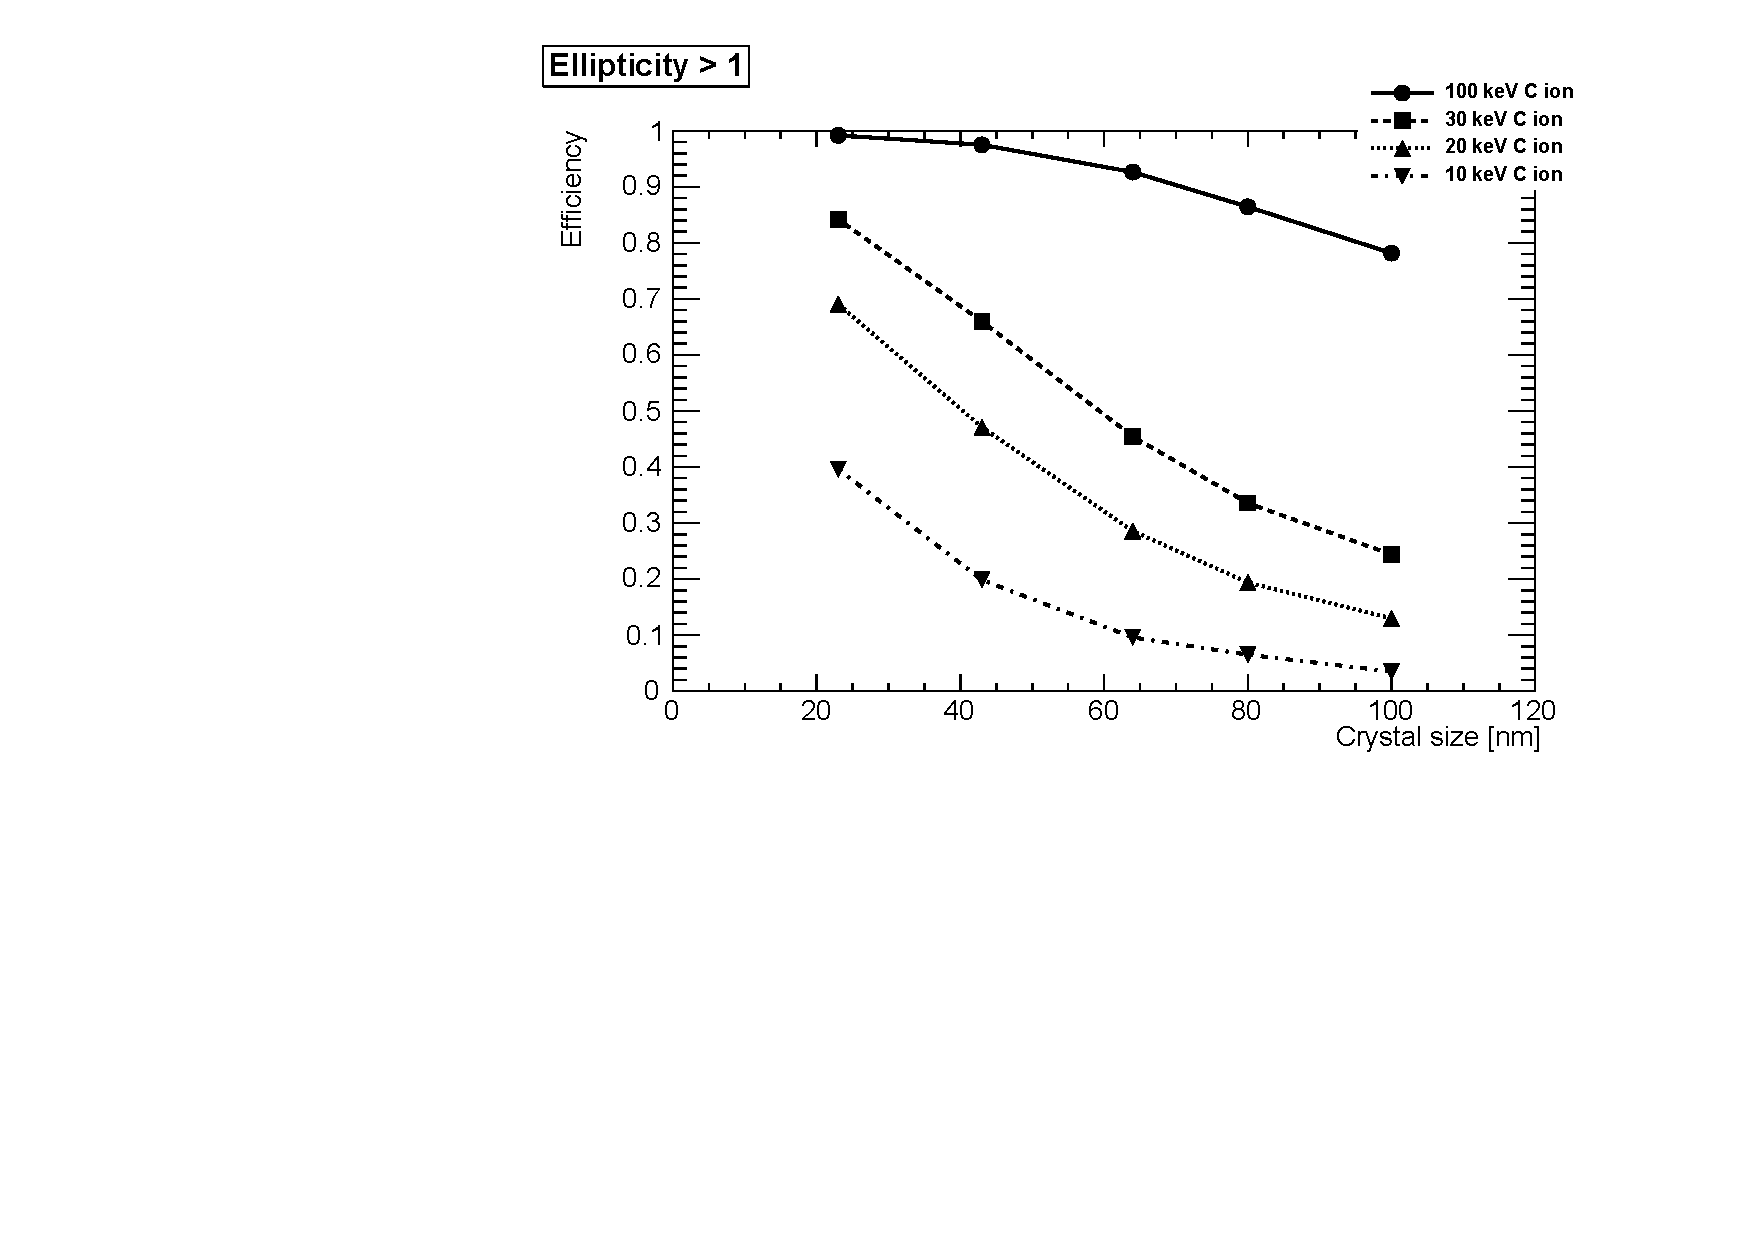
\includegraphics[width=70mm]{./figs/result2.pdf}
\caption{幅70mmで画像を表示する方法\label{fig:test_image}}
\end{figure}
\end{verbatim}

これを実際に描くと図~\ref{fig:test_image}のようになる。

\begin{figure}[htbp]
\centering
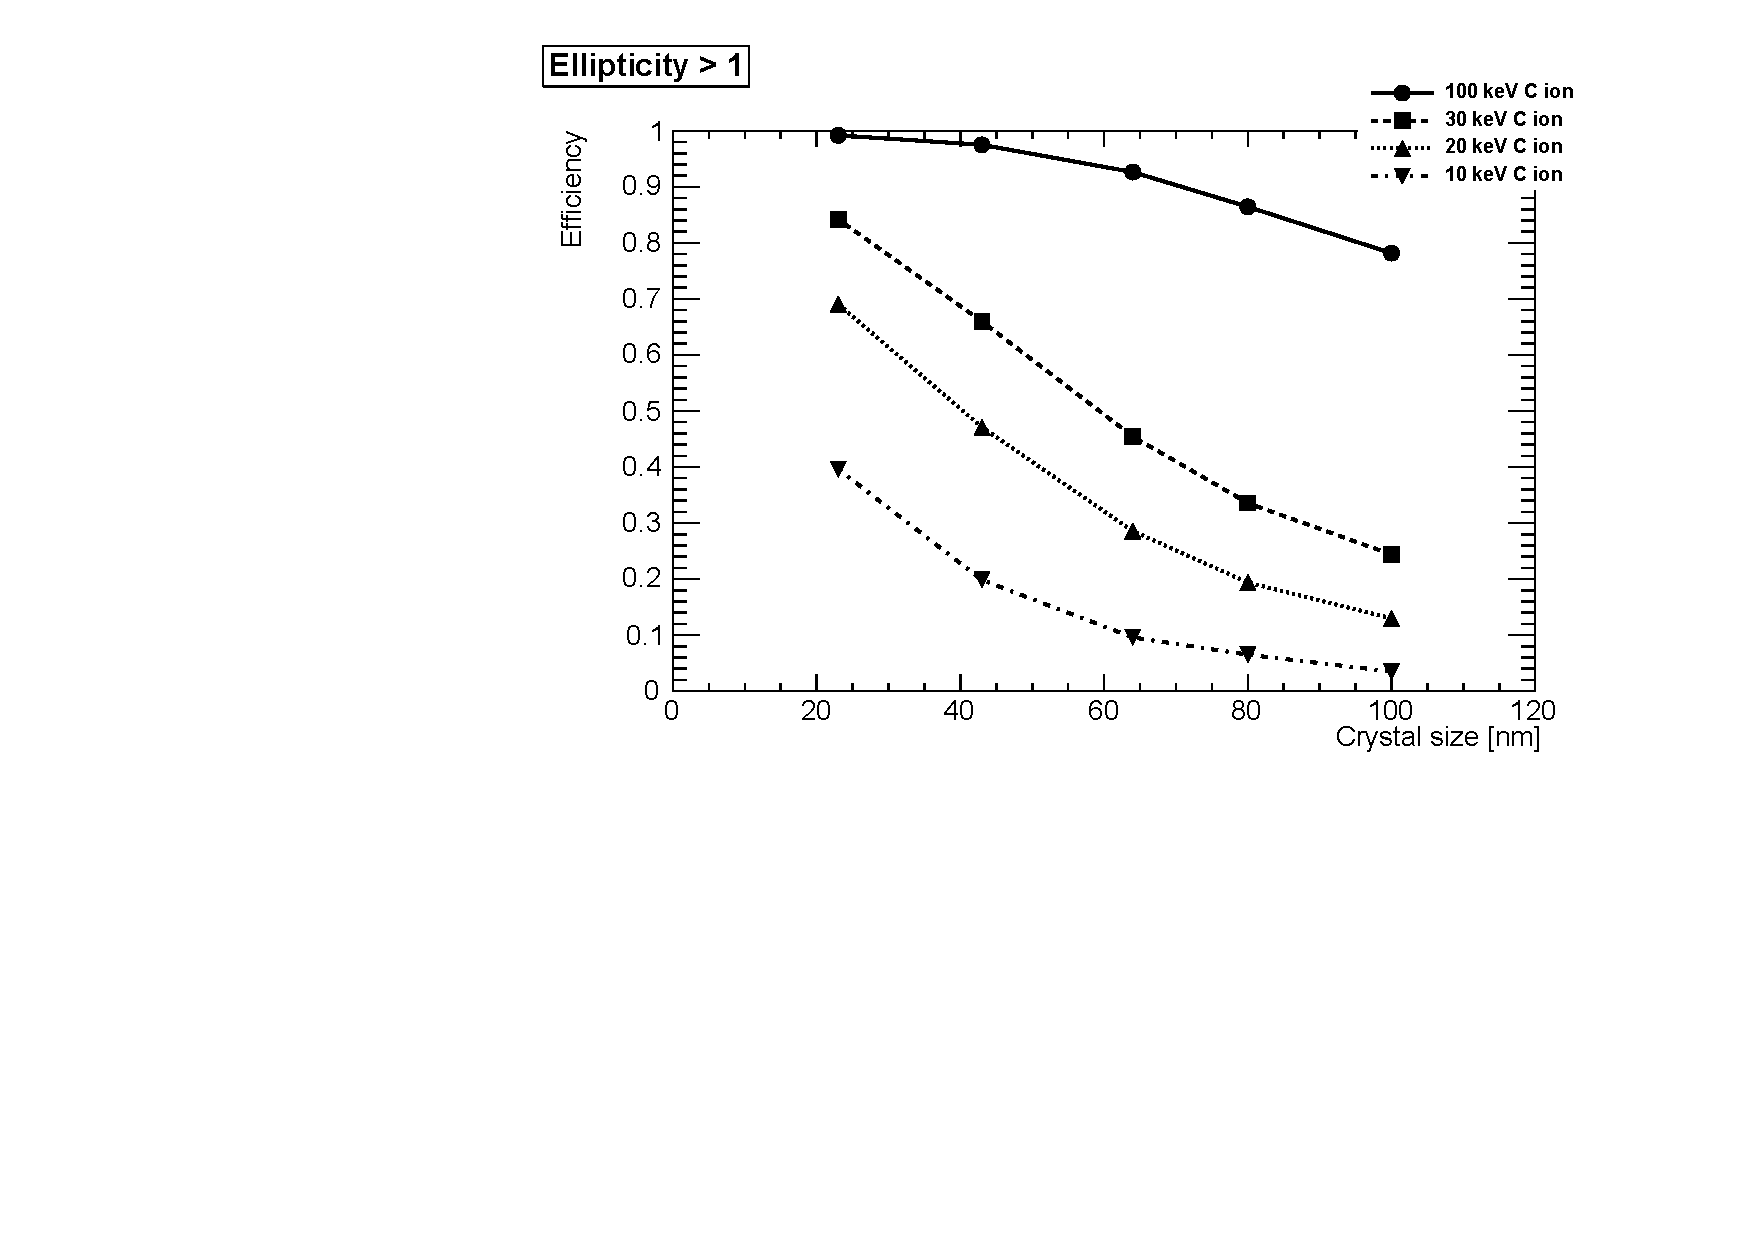
\includegraphics[width=70mm]{./figs/result2.pdf}
\caption{幅70mmで画像を表示する方法\label{fig:test_image}}
\end{figure}

画像のサイズの指定方法は、いくつかの方法がある。

\begin{verbatim}
width=100mm 幅をミリメートルで指定する方法
width=1.0\textwidth テキスト幅からの倍率で指定する方法
scale=0.2 画像やPDFファイルのサイズからの倍率を指定する方法
\end{verbatim}

\section{複数の図を表示}
複数の画像を一つの図に表示させる方法がある。図~\ref{fig:multi_images}で例を描画した。ソース次のとおり。
\begin{verbatim}
\begin{figure}[htbp]
\centering
\subfloat[0~degree]{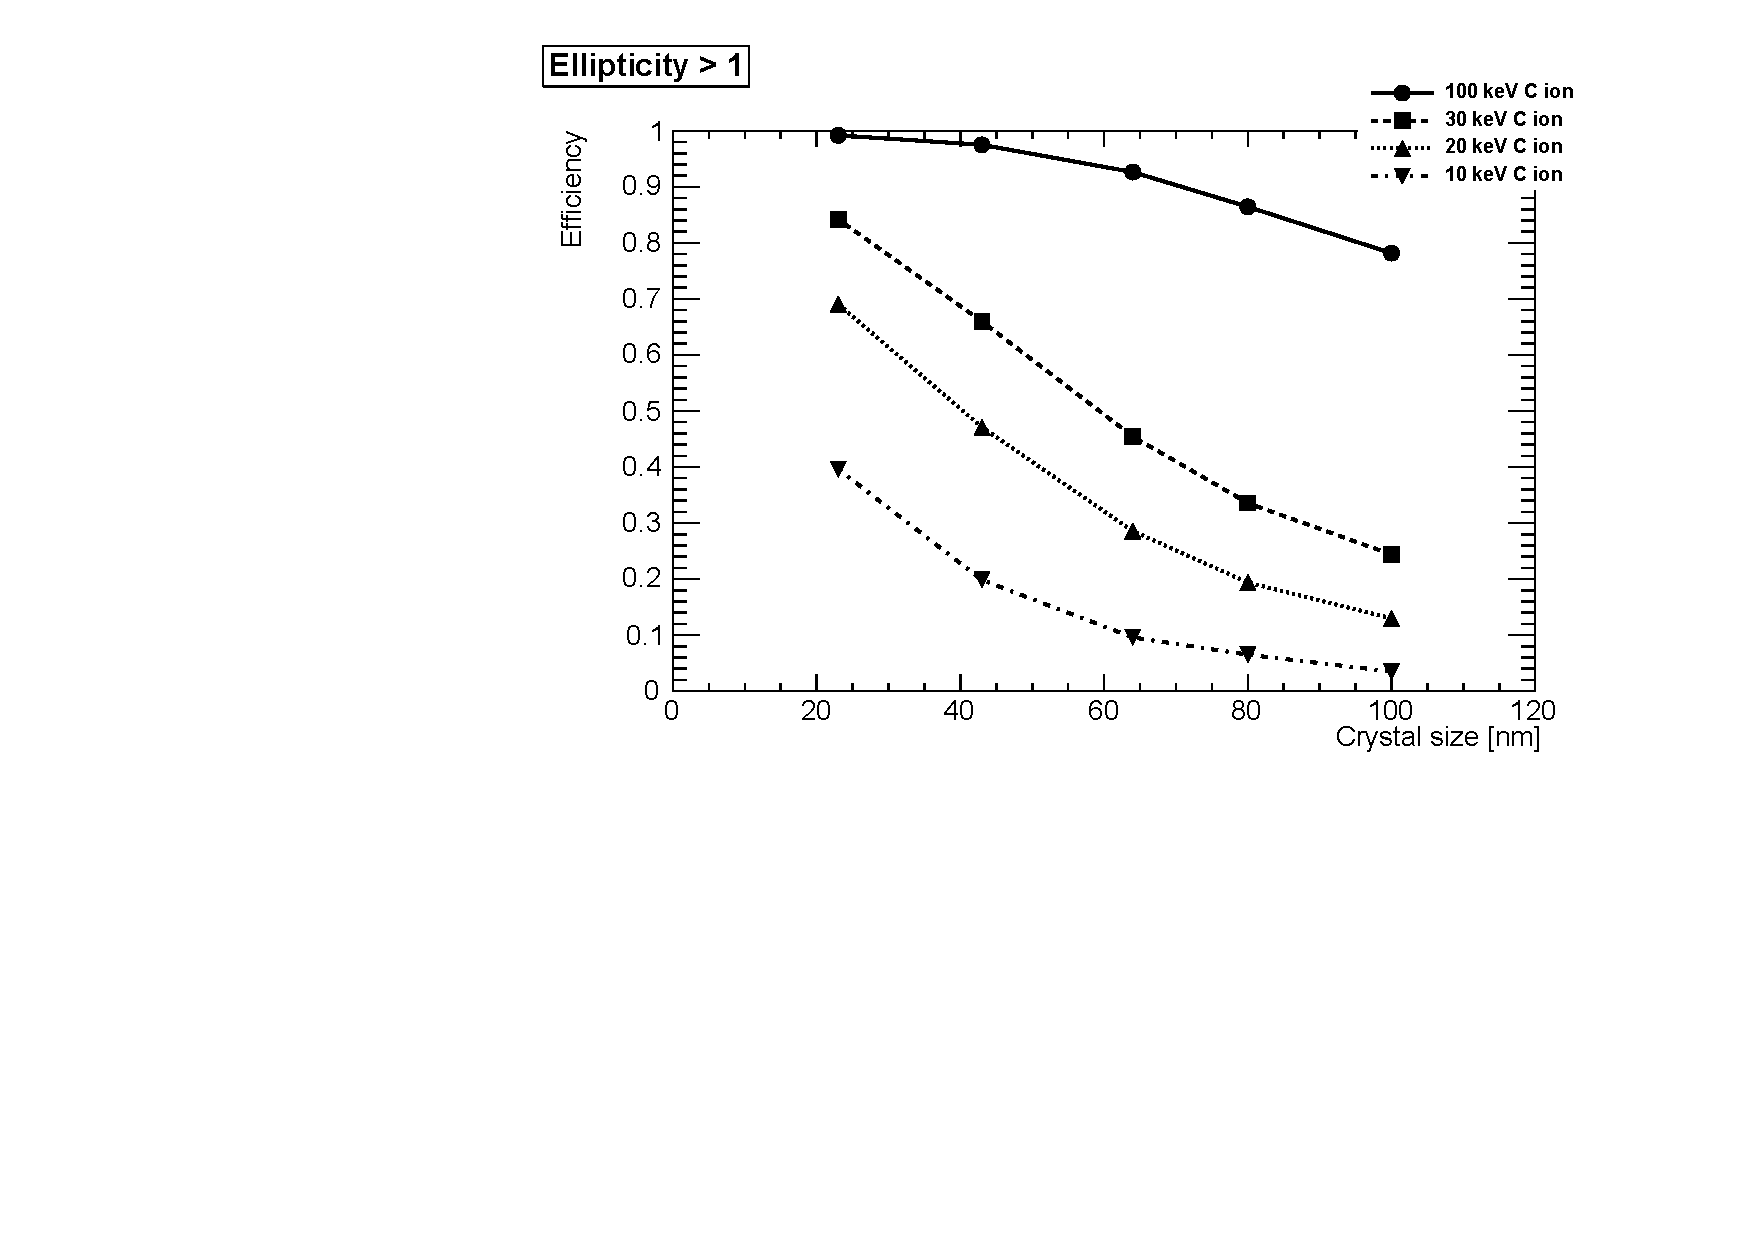
\includegraphics[angle=0,scale=0.2]{./figs/result2.pdf}}
\hspace{1em}
\subfloat[45~degree]{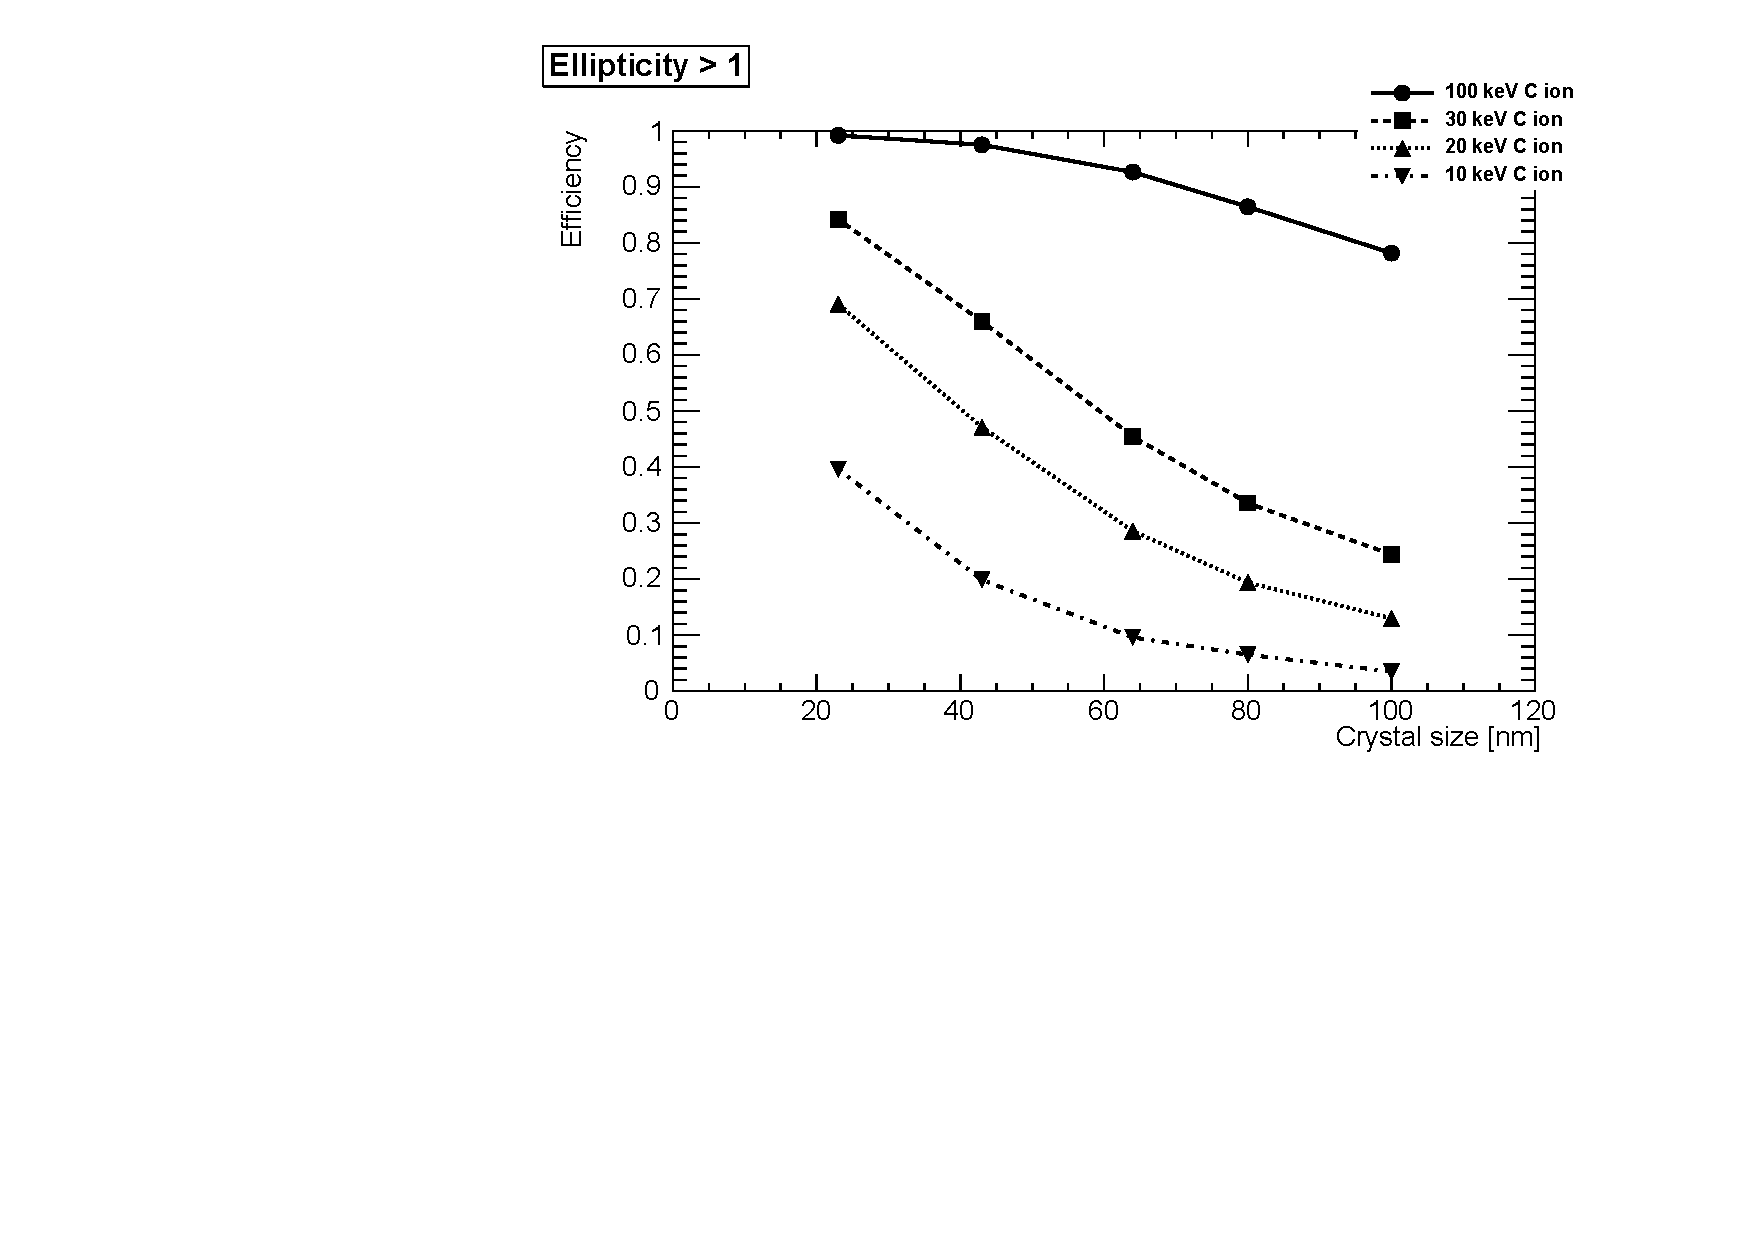
\includegraphics[angle=45,scale=0.2]{./figs/result2.pdf}}
\hspace{1em}
\subfloat[90~degree]{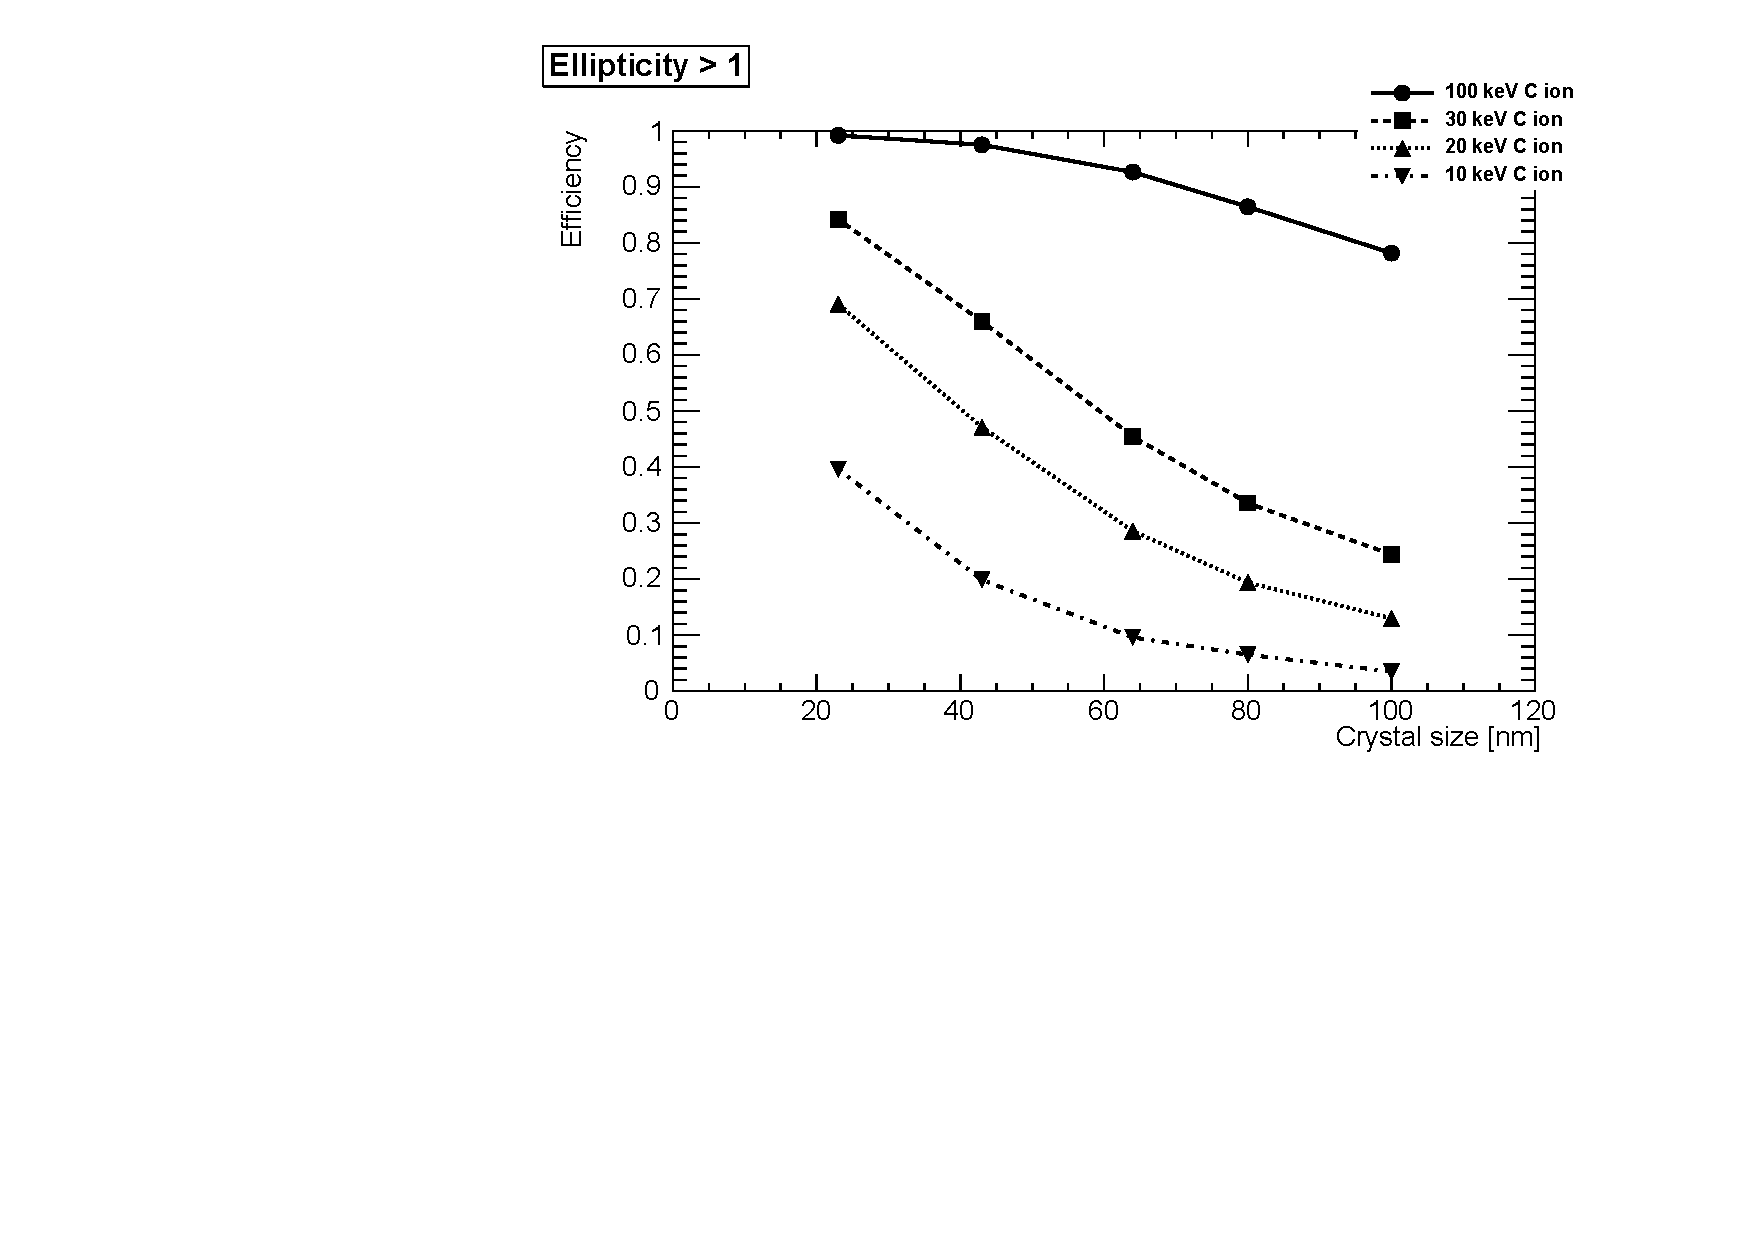
\includegraphics[angle=90,scale=0.2]{./figs/result2.pdf}}
\caption{画像を回転させたり、複数の画像を並べたりする方法\label{fig:multi_images}}
\end{figure}
\end{verbatim}

\begin{figure}[htbp]
\centering
\subfloat[0~degree]{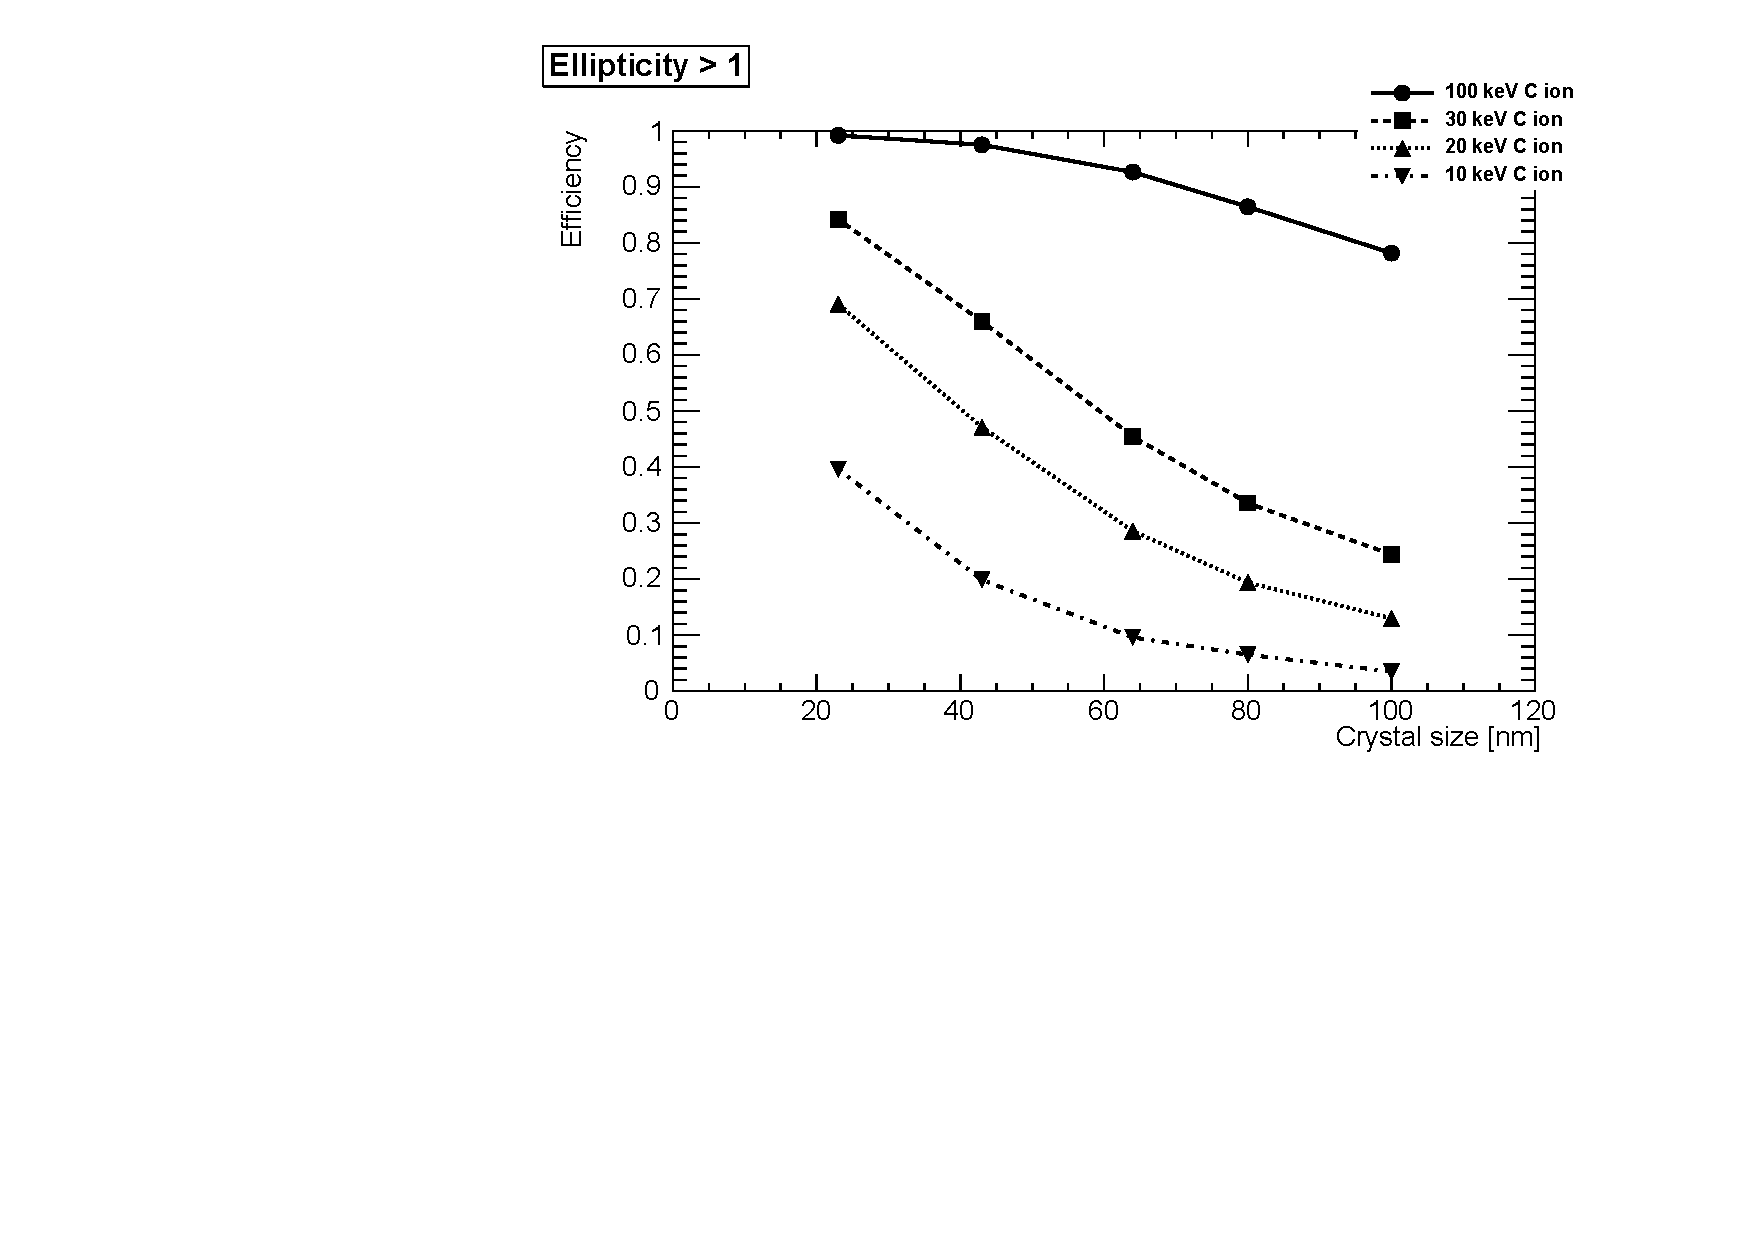
\includegraphics[angle=0,scale=0.2]{./figs/result2.pdf}}
\hspace{1em}
\subfloat[45~degree]{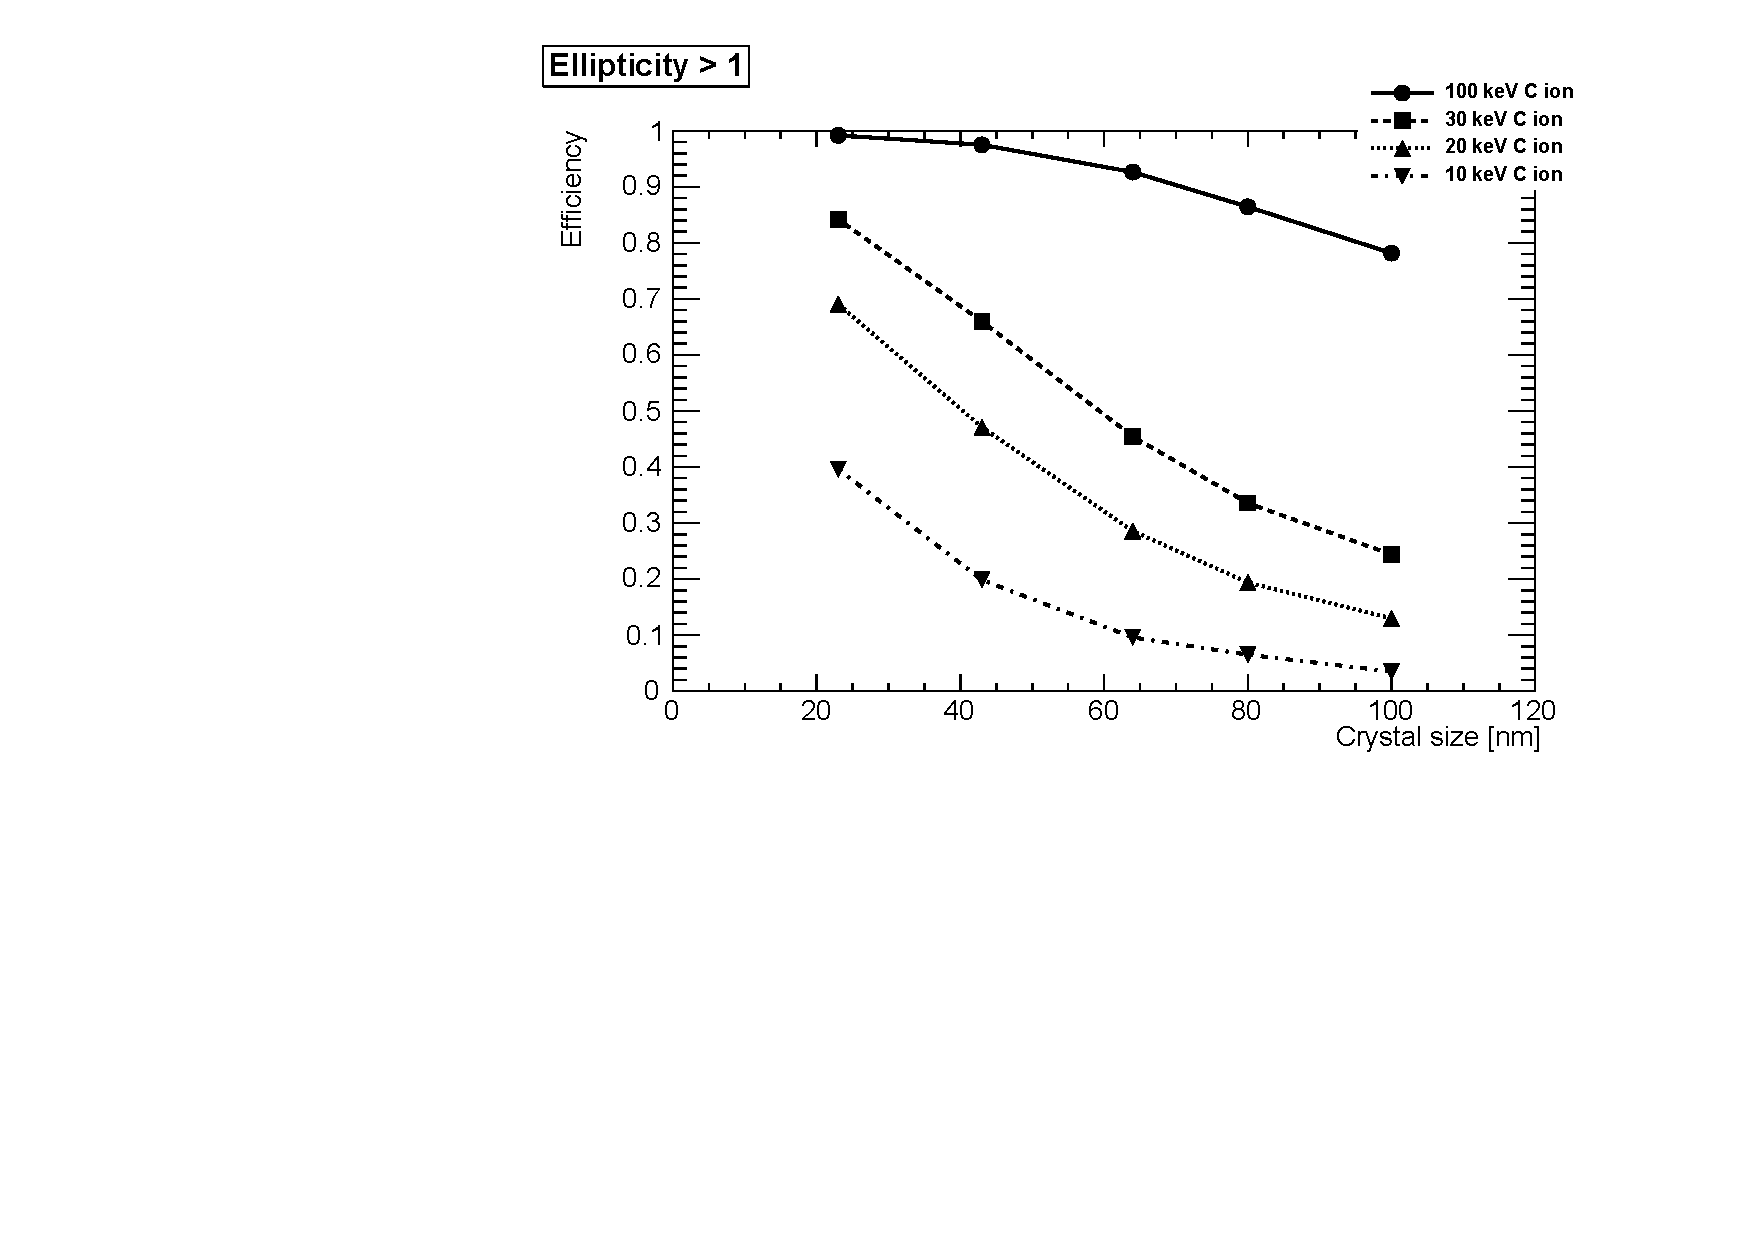
\includegraphics[angle=45,scale=0.2]{./figs/result2.pdf}}
\hspace{1em}
\subfloat[90~degree]{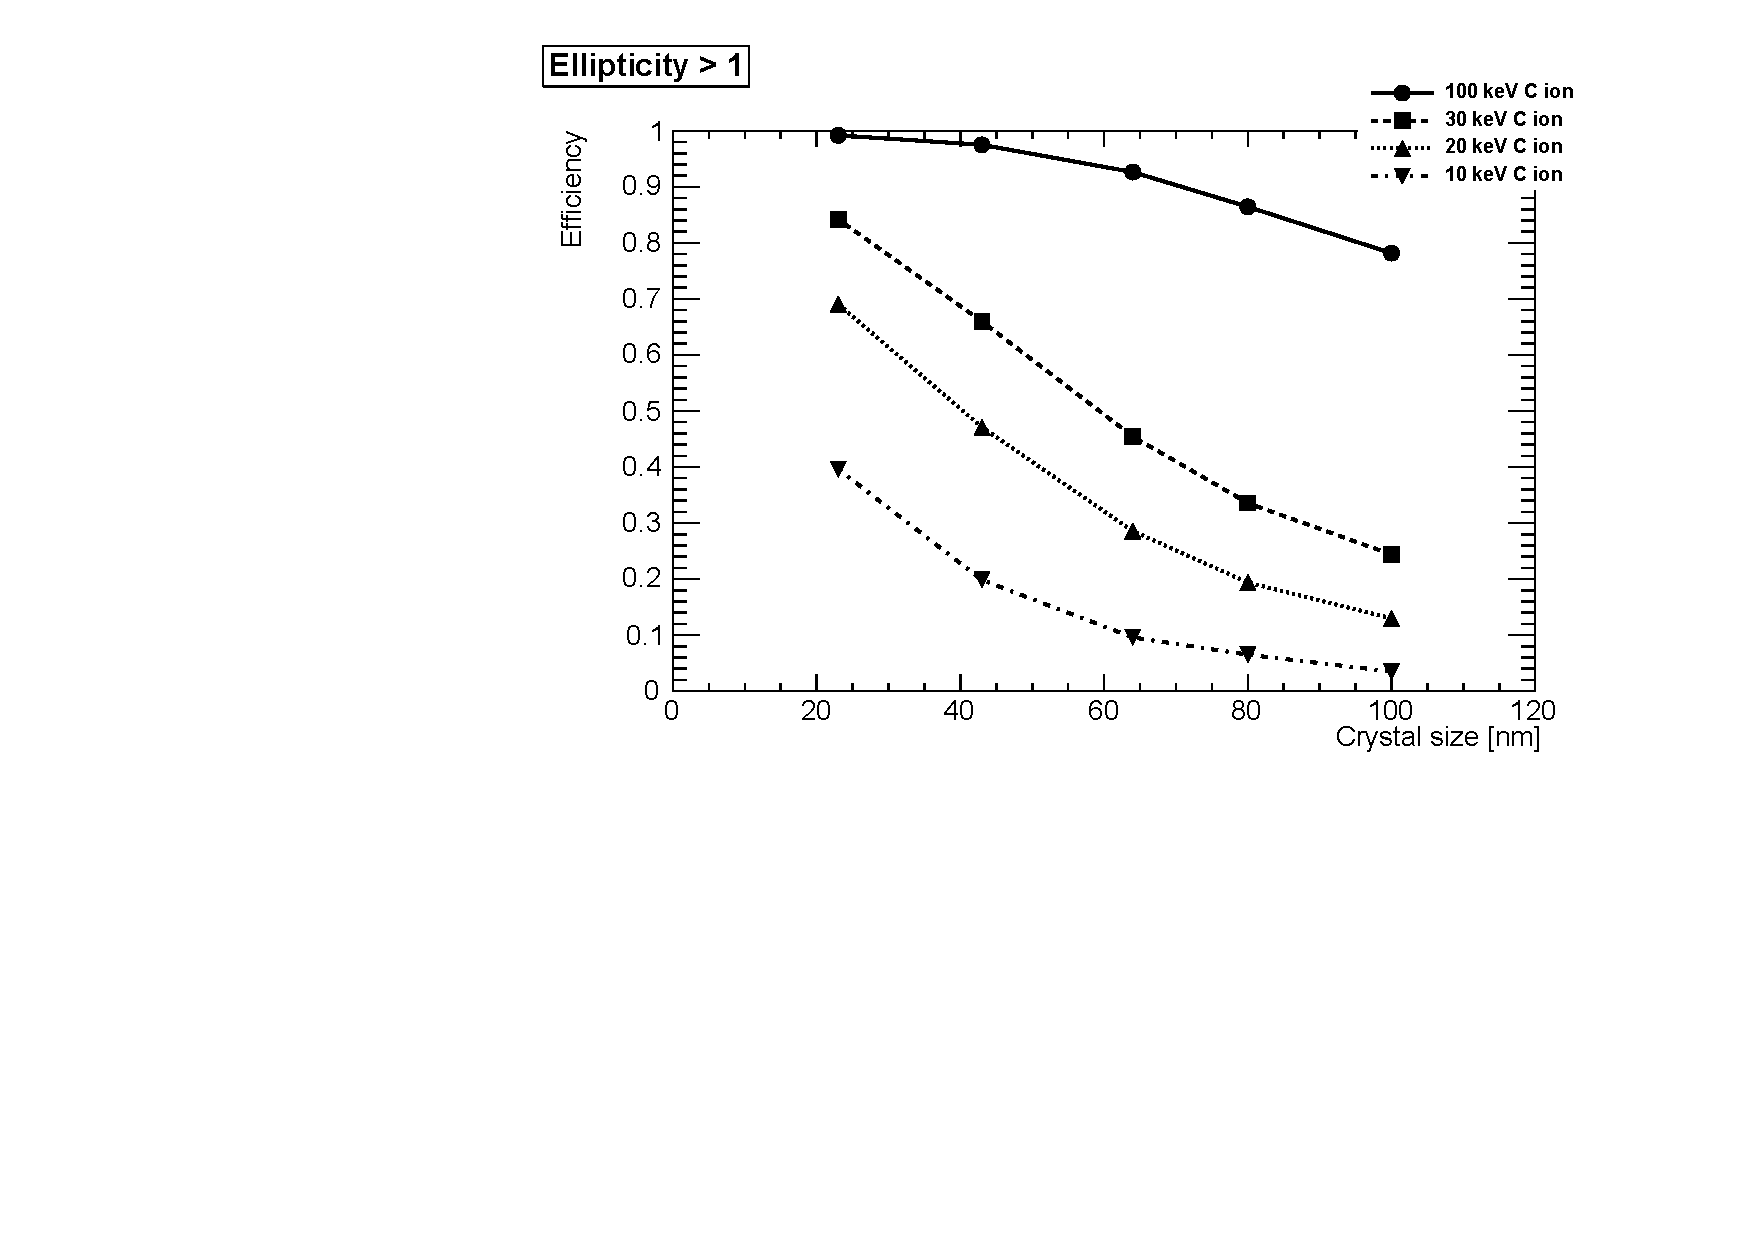
\includegraphics[angle=90,scale=0.2]{./figs/result2.pdf}}
\caption{画像を回転させたり、複数の画像を並べたりする方法\label{fig:multi_images}}
\end{figure}
    

\section{図の表示の応用}

グラフを作るときは、論文内で検索しやすいようにPDFファイルで保存しておくと良い。他の形式ももちろん使える。図~\ref{fig:various_img}で例を描画した。それぞれ異なる拡張子で表示してみた。
ちなみに、png、eps、jpgを使うときは\verb|\usepackage[dvipdfmx]{color}|が必要となる。検索すると分かるが、EPSファイルでは図内の文字が検索可能になっている。

\begin{figure}[htbp]
\centering
\subfloat[pngファイル]{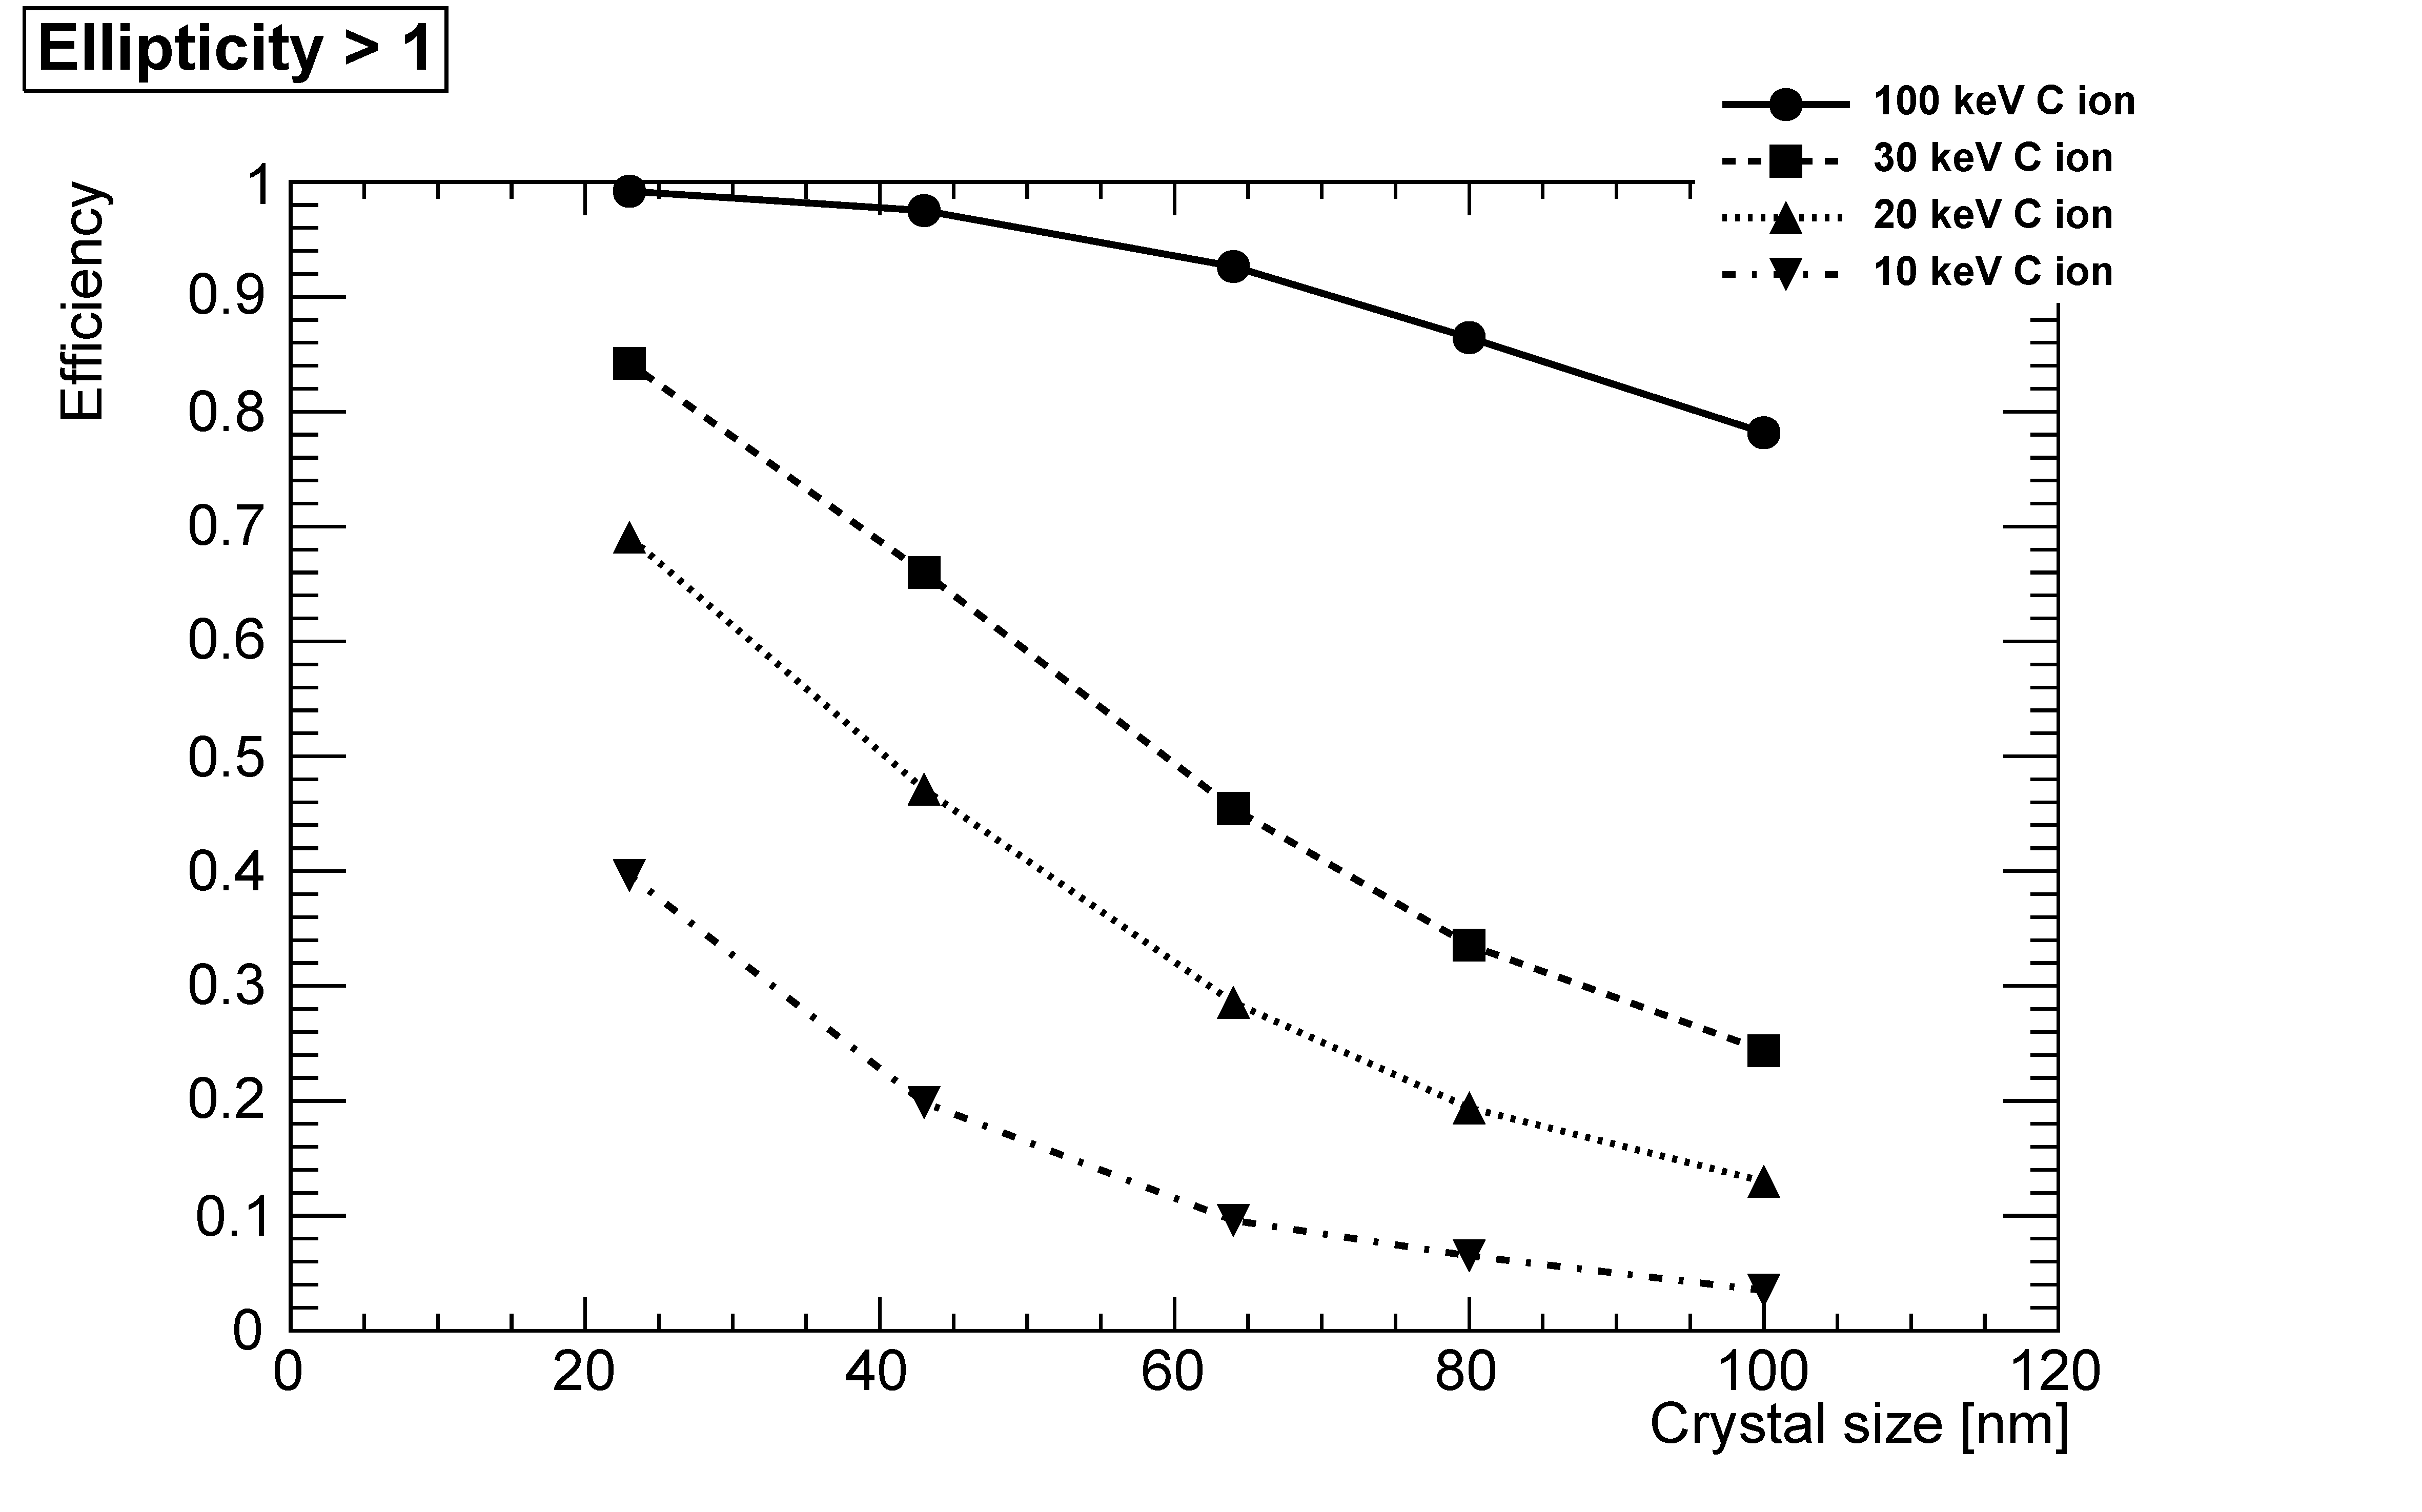
\includegraphics[scale=0.2]{./figs/result.png}}
\subfloat[epsファイル]{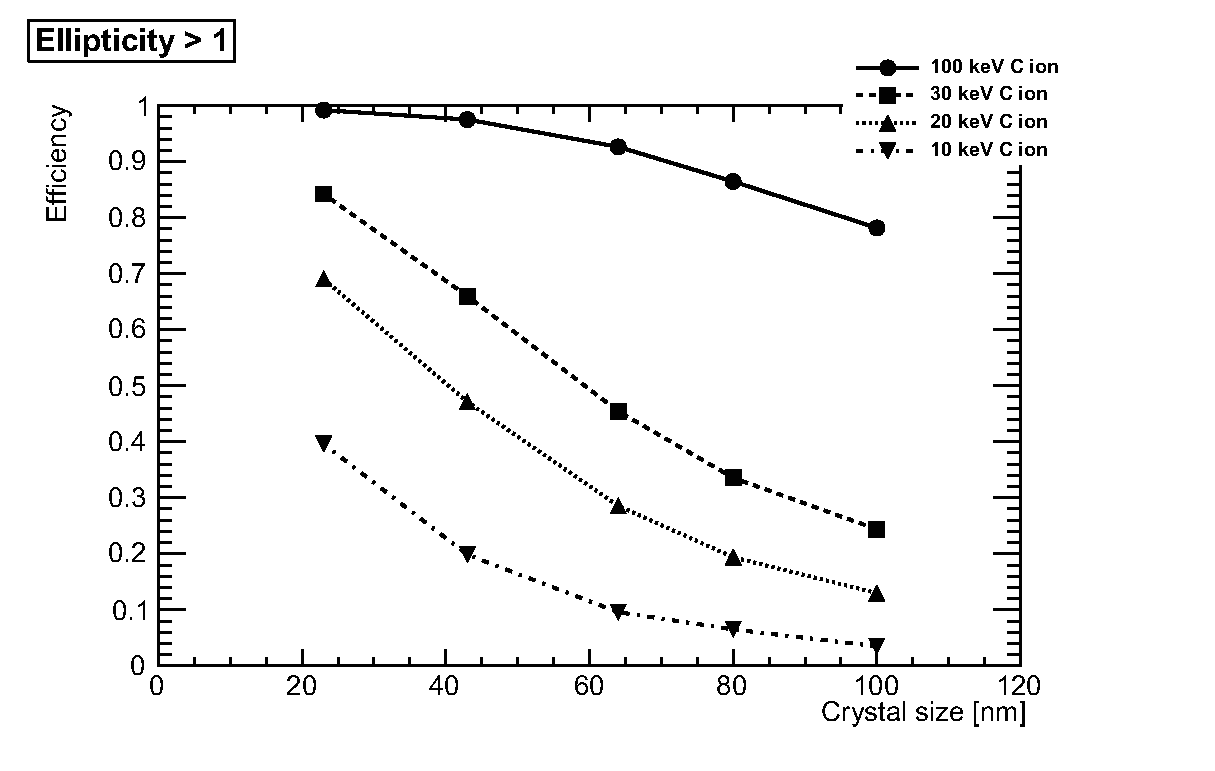
\includegraphics[scale=0.2]{./figs/result.eps}}
\subfloat[jpgファイル]{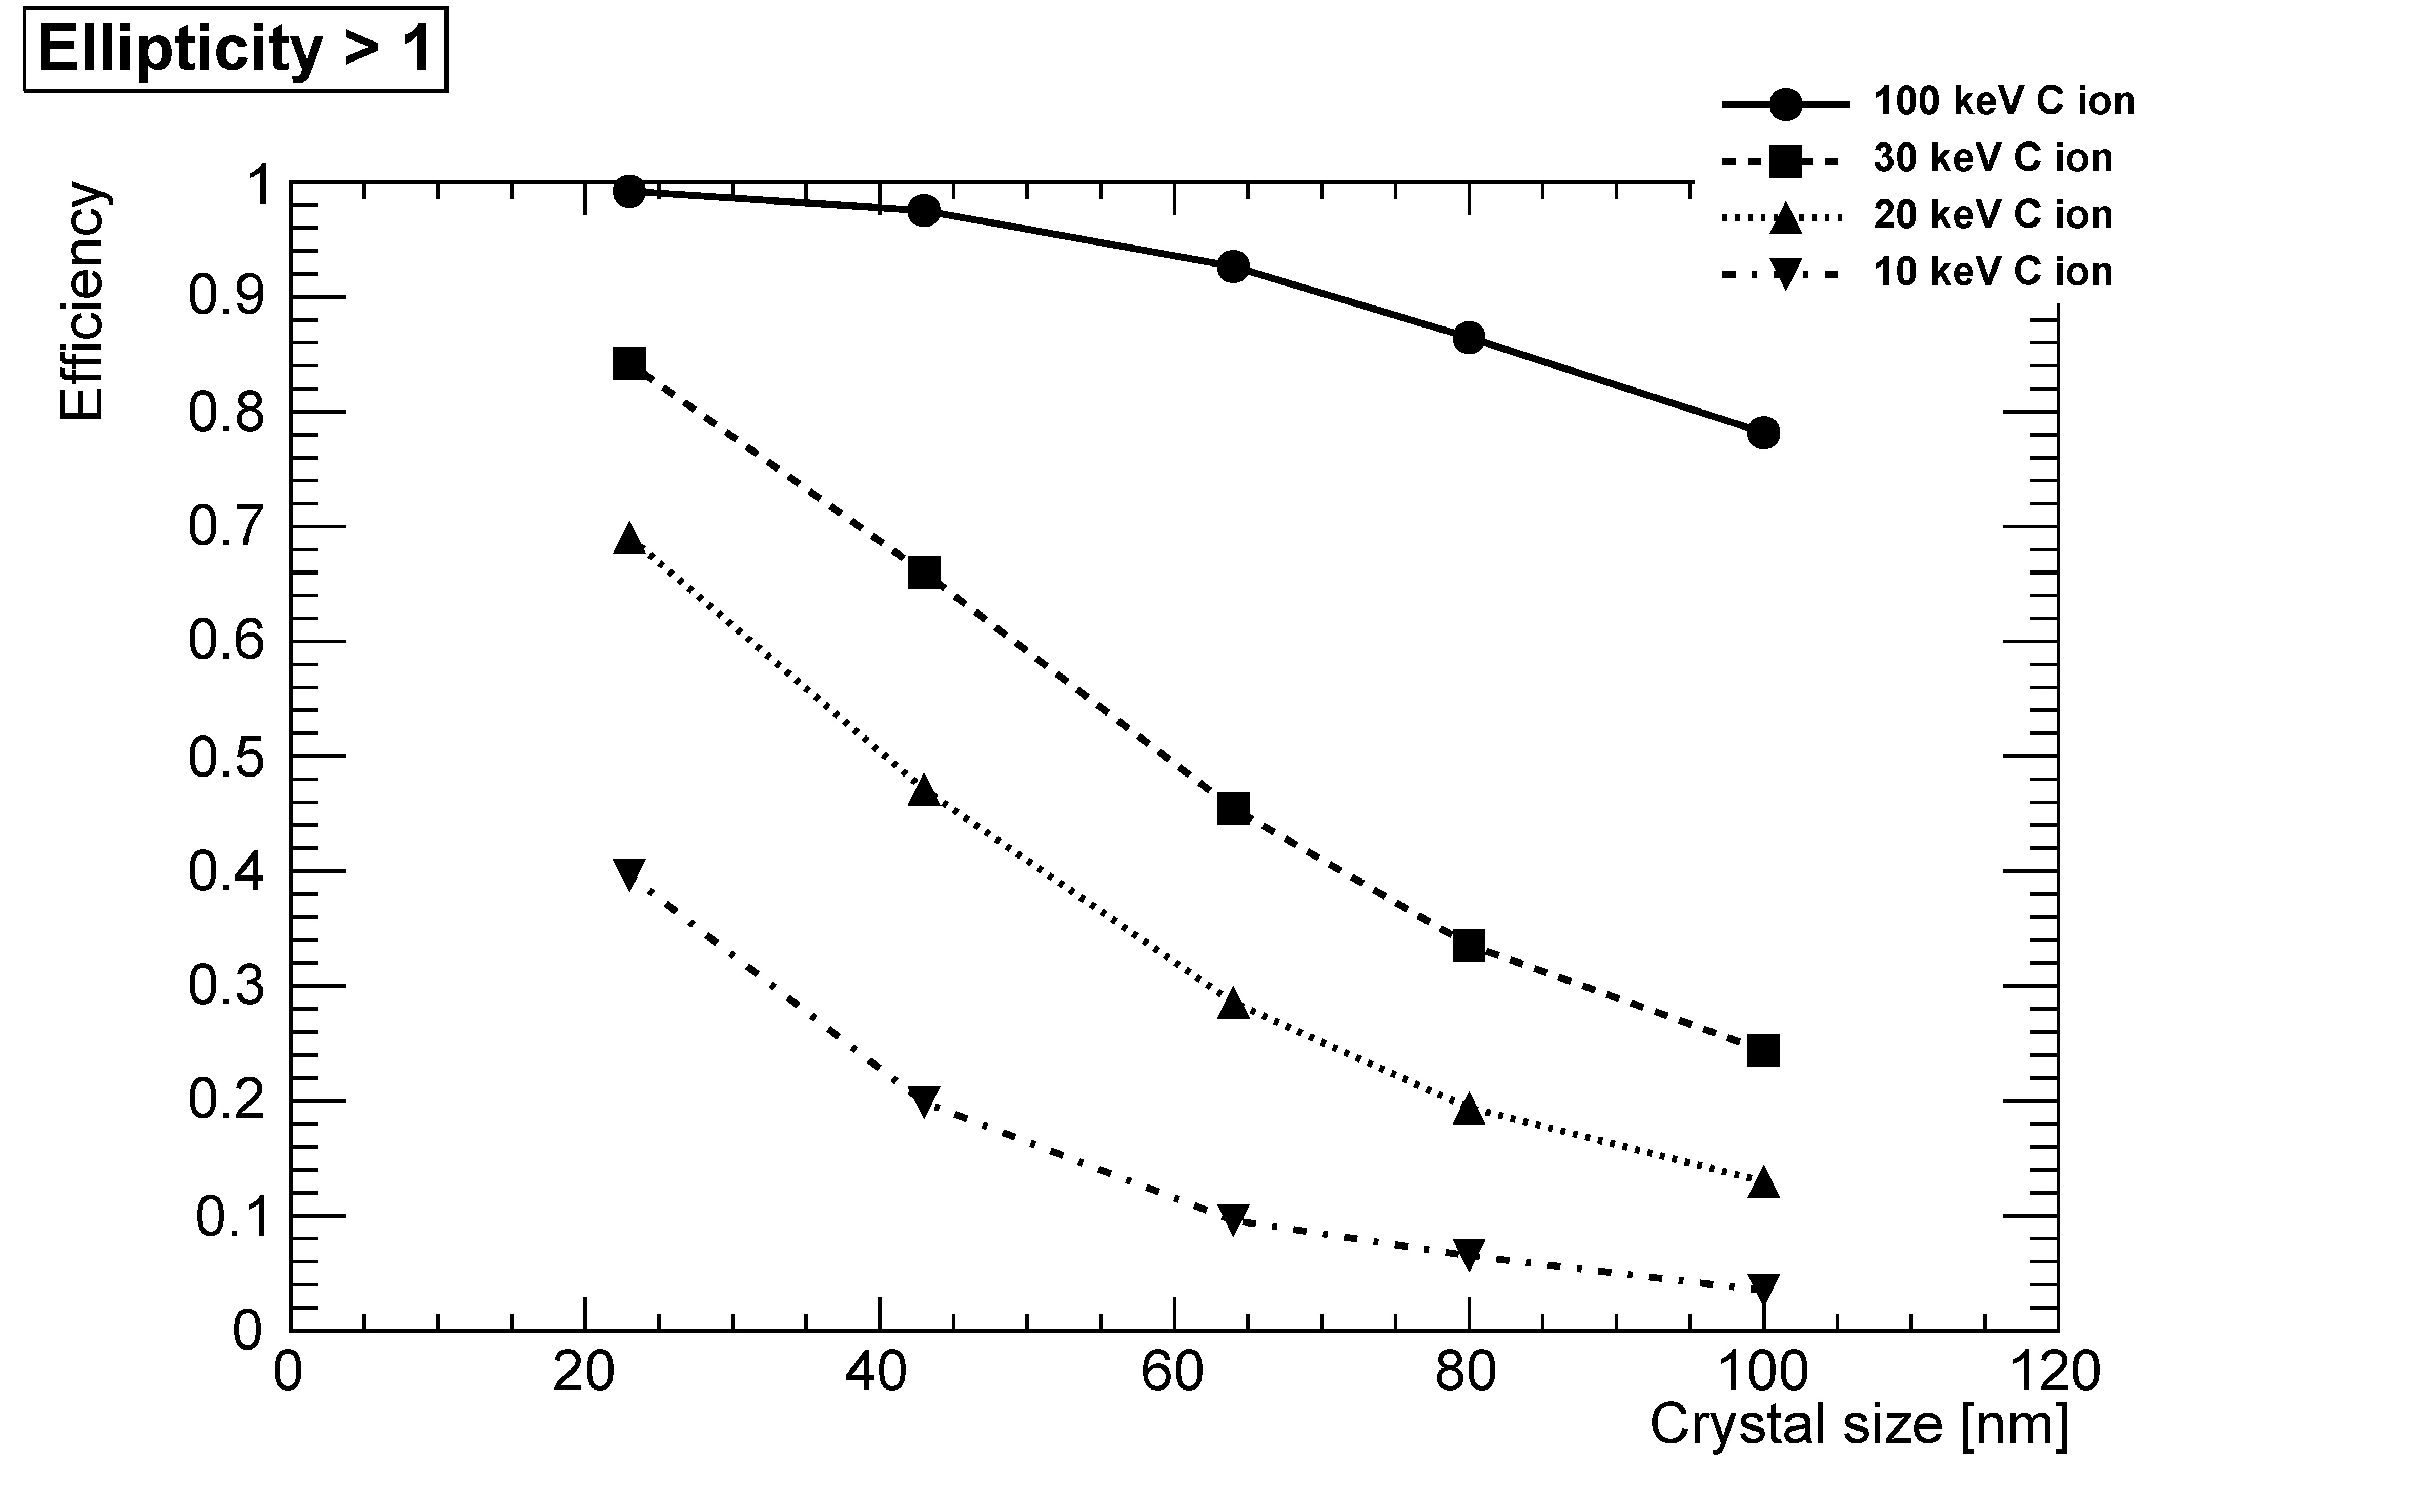
\includegraphics[scale=0.2]{./figs/result.jpg}}
\caption{png, eps, jpgの画像を表示する方法\label{fig:various_img}}
\end{figure}

機会は少ないとは思うが、複数ページを持つPDFはページ番号を指定して表示させることが可能である。図~\ref{fig:multi_page}で例を描画した。図~\ref{fig:page1}は1ページ目、図~\ref{fig:page2}は2ページ目。

\begin{figure}[htbp]
\centering
\subfloat[multi\_page.pdfの1ページ目 width=0.5\label{fig:page1}]
{\fbox{
\includegraphics[page=1,width=0.5\textwidth]{./figs/multi_page.pdf}}}
\hspace{1em}
\subfloat[multi\_page.pdfの2ページ目 width=0.3\label{fig:page2}]
{\fbox{
\includegraphics[page=2,width=0.3\textwidth]{./figs/multi_page.pdf}}}
\caption{複数ページを持つPDFの一部を表示させる方法\label{fig:multi_page}}
\end{figure}

\clearpage

\chapter{表(テーブル)}
\section{texにおける表の書き方}
表は、次の記述で表~\ref{tab:emulsion_telescope}のようになる。詳細はググってほしい。
\begin{verbatim}
\begin{table}[htbp]
\centering
\caption{表の例: GRAINEエマルション望遠鏡の基本性能とFermi-LATとの比較\label{tab:emulsion_telescope}}
\begin{tabular}{r||c|l}
右寄せ&中央寄せ&左寄せ\\
     &Fermi-LAT&GRAINE\\
\hline
\hline
角度分解能@100~MeV& 105~mrad (6.0$^\circ$ )   & 17~mrad (1.0$^\circ$ ) \\
@1~GeV           & 16~mrad(0.90$^\circ$ )    & 1.7~mrad(0.10$^\circ$) \\
検出エネルギー範囲 &20--300~MeV                 & 10~MeV--100~GeV        \\
偏光感度          &無                          &有                      \\
不感時間          &26.5~$\mu$sec (readout time)& 0\%                    \\
\hline
\end{tabular}
\end{table}
\end{verbatim}
\begin{table}[htbp]
\centering
\caption{表の例: GRAINEエマルション望遠鏡の基本性能とFermi-LATとの比較\label{tab:emulsion_telescope}}
\begin{tabular}{r||c|l}
右寄せ&中央寄せ&左寄せ\\
     &Fermi-LAT&GRAINE\\
\hline
\hline
角度分解能@100~MeV& 105~mrad (6.0$^\circ$ )   & 17~mrad (1.0$^\circ$ ) \\
@1~GeV           & 16~mrad(0.90$^\circ$ )    & 1.7~mrad(0.10$^\circ$) \\
検出エネルギー範囲 &20--300~MeV                 & 10~MeV--100~GeV        \\
偏光感度          &無                          &有                      \\
不感時間          &26.5~$\mu$sec (readout time)& 0\%                    \\
\hline
\end{tabular}
\end{table}

\section{Excelでテーブルを作ってtexに挿入する方法}
複雑なレイアウトの表を作るときは、texファイル上で格闘するよりもMicrosoft Excelなどで作成した方が楽なことが多い。
例えば、セル内で改行したいとき、右寄せ中央寄せなどを同じ列で異なる設定にしたいとき、罫線を好きな場所に引きたい時、セルを結合したいときなどである。

Excelで表を作成し、PDFファイルとして保存し、必要な場所だけを切り抜いて画像またはPDFファイルとして保存する。そのPDFファイル(画像)を\ref{sec:figure}で説明したように図として挿入する。そのとき、\verb|\begin{figure} ~~ \end{figure}| ではなく\verb|\begin{table} ~~ \end{table}| とすると、図~1、図~2ではなく、表~1、表~2と自動的に番号付けされる。

Excelからtexファイルに表を挿入はいくつかの工程が必要となる。
表~\ref{tab:table_cop}に各方法をまとめた。
pdfcropを使うときは、Perlというプログラムを事前にインストールする必要がある(WindowsユーザーだとStrawberry Perl)。

\begin{verbatim}
\begin{table}[htbp]
    \centering
    \caption{\LaTeX で表を作成する方法(これはLaTeX+PDF)\label{tab:table_cop}}
    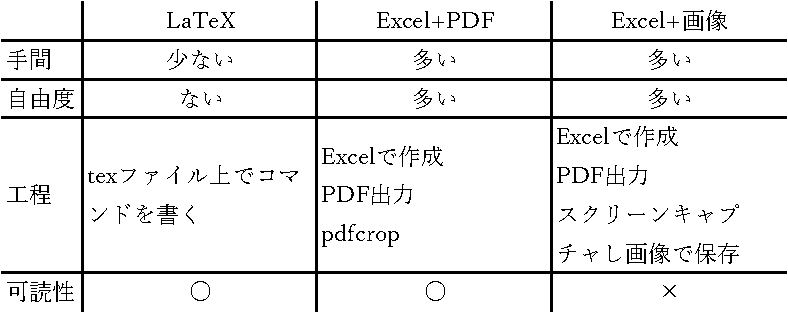
\includegraphics[width=110mm]{./figs/table_crop.pdf}
\end{table}
\end{verbatim}
\begin{table}[htbp]
    \centering
    \caption{\LaTeX で表を作成する方法(これはLaTeX+PDF)\label{tab:table_cop}}
    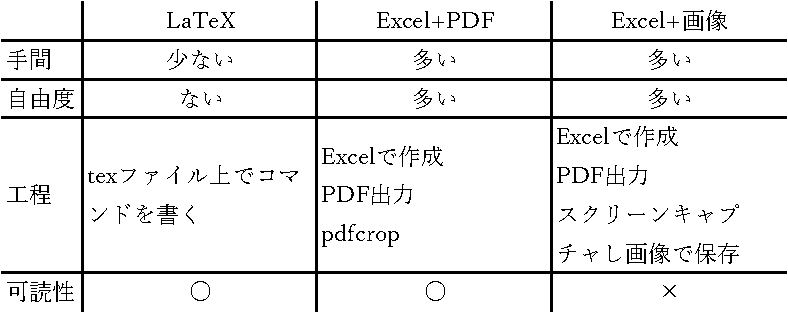
\includegraphics[width=110mm]{./figs/table_crop.pdf}
\end{table}
    
\section{画像を文字の横に置く方法}

表の機能を使って、画像を文字の横に置くことも可能である。ただし、あまり多用するものではない。
図~\ref{fig:curry_rice}のように左側に簡単な文章を置き、右側に画像を置くといったことも可能である。
書き方はソースを参照せよ。

\begin{figure}[htbp]
    \begin{tabular}{lr}
        \begin{tabular}{l}
            カレーの作り方\\
            ・欲しい材料を欲しいサイズに切る\\
            ・腐食と熱に強い金属製の容器に水と切った材料を入れる\\
            ・容器の下から加熱する\\
            ・辛い薬剤を適量入れる\\
            ・米と水をライスクッカーに入れ電源を入れ完成まで待つ\\
            ・陶器製の容器に完成した米と金属製容器で加熱された混合物を盛る\\
        \end{tabular}& 
        \begin{minipage}{40mm}{
            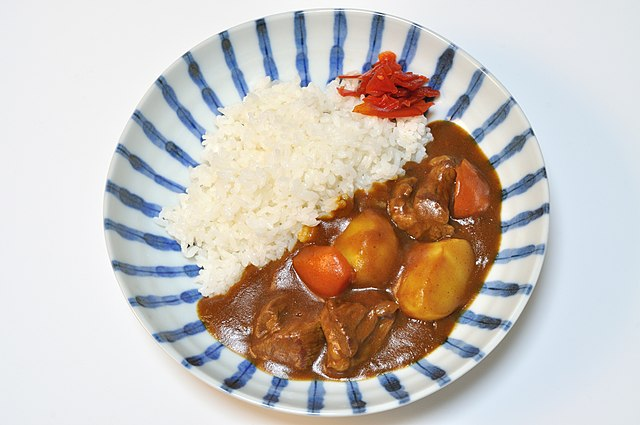
\includegraphics[width=40mm]{./figs/curry_rice.jpg}
            \caption{一般的にカレーライスと呼ばれる食べ物\label{fig:curry_rice}}
        }\end{minipage}\\
    \end{tabular}
\end{figure}

\chapter{リスト}
幾つかのリストを書く方法を示す。itemize, enumerate, descriptionがよく使われる。
\section{itemizeを使う方法}
\begin{verbatim}
\begin{itemize}
 \item 調液
 \item 粒子形成
 \item 水洗+脱塩
\end{itemize}
\end{verbatim}

\begin{itemize}
 \item 調液
 \item 粒子形成
 \item 水洗+脱塩
\end{itemize}
\section{descriptionを使う方法}
\begin{verbatim}
\begin{description}
 \item [調液]\mbox{} \\調液とは、
 \item [粒子形成]\mbox{} \\粒子形成とは、
 \item [水洗+脱塩]\mbox{} \\水洗と脱塩とは、
\end{description}
\end{verbatim}
\begin{description}
 \item [調液]\mbox{} \\調液とは、
 \item [粒子形成]\mbox{} \\粒子形成とは、
 \item [水洗+脱塩]\mbox{} \\水洗と脱塩とは、
\end{description}
\section{enumerateを使う方法}
原子核乳剤の主な原料は・・・番号を1番以外から始めたいときは\verb|\setcounter{enumi}{X}|を使う。
\begin{verbatim}
\begin{enumerate}
\setcounter{enumi}{10}
 \item 硝酸銀 (高い)
 \item 臭化カリウム
\end{enumerate}
\end{verbatim}
\begin{enumerate}
\setcounter{enumi}{10}
 \item 硝酸銀 (高い)
 \item 臭化カリウム
\end{enumerate}

\chapter{数式}
equation*コマンドで数式を書くとただの数式を書ける。
\begin{verbatim}
\begin{equation*}
a=b
\end{equation*}
\end{verbatim}
\begin{equation*}
a=b
\end{equation*}
equationコマンドで数式を書くと番号が付く。式~\ref{equ:ab}で例を示す。
\begin{verbatim}
\begin{equation}
a=b
\label{equ:ab}
\end{equation}
\end{verbatim}
\begin{equation}
a=b
\label{equ:ab}
\end{equation}
一粒子系のシュレーディンガー方程式を式~\ref{equ:oneparticle}で示す。
\begin{verbatim}
\begin{equation}
i\hbar\frac{\partial}{\partial t} \psi(\boldsymbol{x},t) = 
\left [ \frac{-\hbar^2}{2m}\nabla^2 + V(\boldsymbol{x},t)\right ] \psi(\boldsymbol{x},t)
\label{equ:oneparticle}
\end{equation}
\end{verbatim}
\begin{equation}
i\hbar\frac{\partial}{\partial t} \psi(\boldsymbol{x},t) = 
\left [ \frac{-\hbar^2}{2m}\nabla^2 + V(\boldsymbol{x},t)\right ] \psi(\boldsymbol{x},t)
\label{equ:oneparticle}
\end{equation}

\section{上付き下付き文字}
\begin{verbatim}
$x^a, x^{a+b}, x^{a^b}, a_i, a_{ij}, a_{i_j}$
\end{verbatim}
$x^a, x^{a+b}, x^{a^b}, a_i, a_{ij}, a_{i_j}$

\section{不等号}
\begin{verbatim}
$\sim, \simeq, >, <, \geq, \leq, \gg, \ll$
\end{verbatim}
$\sim, \simeq, >, <, \geq, \leq, \gg, \ll$

\section{演算子}
\begin{verbatim}
$+, -, \times, \div, \pm, \mp, \circ, \cdot$
\end{verbatim}
$+, -, \times, \div, \pm, \mp, \circ, \cdot$

\section{平方根}
\begin{verbatim}
$\sqrt{x}, \sqrt[n]{x}$
\end{verbatim}
$\sqrt{x}, \sqrt[n]{x}$

\section{ギリシャ文字}
\begin{verbatim}
$\Gamma, \Delta, \Theta, \Lambda, \Xi, \Pi, \Sigma, \Upsilon, \Phi, \Psi, \Omega$
\end{verbatim}
$\Gamma, \Delta, \Theta, \Lambda, \Xi, \Pi, \Sigma, \Upsilon, \Phi, \Psi, \Omega$

\begin{verbatim}
$\alpha, \beta, \gamma, \delta, \epsilon, \zeta, \eta, \theta, \iota, \kappa, \lambda, $\\
$\mu, \nu, $\xi, o, \pi, \rho, \sigma, \tau, \upsilon, \phi, \chi, \psi, \omega, $
\end{verbatim}
$\alpha, \beta, \gamma, \delta, \epsilon, \zeta, \eta, \theta, \iota, \kappa, \lambda, $\\
$\mu, \nu, \xi, o, \pi, \rho, \sigma, \tau, \upsilon, \phi, \chi, \psi, \omega, $
\section{行列}
\begin{verbatim}
\begin{equation}
 \begin{array}{rrr}
-1 & \ldots & 3 \\
\vdots & \ddots & 600 \\
  7 & 8 & -9
 \end{array}
\end{equation}
\end{verbatim}

\begin{equation}
\begin{array}{rrr}
-1 & \ldots & 3 \\
\vdots & \ddots & 600 \\
7 & 8 & -9
\end{array}
\end{equation}
\section{括弧(かっこ)}
\verb|\left \right|を使うと\verb|[ ], ( ), { }, | $|\;|$等で囲まれる数式を正しく囲むことができる。
\verb|{ }|は数式内でのメタ文字なので、数式内では\verb|\{ \}|と書く。
\begin{verbatim}
 \left [ \frac{0}{1} \right ] + [\frac{0}{1}]
 \left ( \frac{0}{1} \right ) + (\frac{0}{1})
 \left \{ \frac{0}{1} \right \} + \{\frac{0}{1}\}
 \left | \frac{0}{1} \right | + |\frac{0}{1}|
\end{verbatim}
\begin{equation}\left [ \frac{0}{1} \right ] + [\frac{0}{1}]\end{equation}
\begin{equation}\left ( \frac{0}{1} \right ) + (\frac{0}{1})\end{equation}
\begin{equation}\left \{ \frac{0}{1} \right \} + \{\frac{0}{1}\}\end{equation}
\begin{equation}\left | \frac{0}{1} \right | + |\frac{0}{1}|\end{equation}
\section{数式中の空白や改行}
数式モードでは全ての空白は無視されるので、明示的に空白コマンドを使う。改行して=でそろえたい場合は\verb|\begin{split}\end{split}|を使い、\verb|\\|で改行、\verb|&|でそろえる場所を指定する。
\begin{verbatim}
\begin{equation}
\begin{split}
a&=|\;| 大きめの空白\\
b&=|\:| 中くらいの空白\\
c&=|\,| 小さめの空白\\
d&=|| 空白なし\\
e&=|\!| 負の空白
\end{split}
\end{equation}
\end{verbatim}
\begin{equation}
\begin{split}
a&=|\;| 大きめの空白\\
b&=|\:| 中くらいの空白\\
c&=|\,| 小さめの空白\\
d&=|| 空白なし\\
e&=|\!| 負の空白
\end{split}
\end{equation}
\section{総和・総乗}
\begin{verbatim}
\begin{equation} f(x) = \sum_{i=0}^n x_i \end{equation}

\begin{equation}  f(x) = \prod_{i=0}^n x_i \end{equation}
\end{verbatim}
\begin{equation} f(x) = \sum_{i=0}^n x_i \end{equation}

\begin{equation}  f(x) = \prod_{i=0}^n x_i \end{equation}
\section{数式装飾}
\subsection{文字へのアクセント}
\noindent
ハット        $\hat{x}$ = \verb|$\hat{x}$|\\
ベクトル       $\vec{x}$ = \verb|$\vec{x}$|\\
ドット(一階微分)   $\dot{x}$ = \verb|$\dot{x}$|\\
二重ドット(二階微分) $\ddot{x}$ = \verb|$\ddot{x}$|\\
ダッシュ       $y'$ = \verb|$y'$|\\
二重ダッシュ     $y''$ = \verb|$y''$|\\
\subsection{数式へのアクセント}
\noindent
ベクトル       $\overrightarrow{ma}$ = \verb|$\overrightarrow{ma}$|\\
上ライン       $\overline{ma}$ = \verb|$\overline{ma}$|\\
\section{頻出表現}
\label{sec:frequent}
\noindent
角度         $^\circ$ = \verb|$^\circ$|\\
ミクロン       $\mu m$ = \verb|$\mu m$|\\
数式中で斜体にしない $\rm{mm}$ = \verb|$\rm{mm}$|\\
ニュートリノ振動   $\nu_{\mu} \rightarrow \nu_{\tau}$ = \verb|$\nu_{\mu} \rightarrow \nu_{\tau}$|\\
臭化銀の沈殿     $\rm{KBr+AgNO_3\rightarrow AgBr\downarrow+KNO_3}$ = \\
\verb|$\rm{KBr+AgNO_3\rightarrow AgBr\downarrow+KNO_3}$|\\
ハイパー核      $_{\Lambda\Lambda}^{~6}$He = \verb|$_{\Lambda\Lambda}^{~6}$He|\\
レイリーの基準    $\delta x = 0.61\frac{\lambda}{\rm{NA}}$ = \verb|$\delta x = 0.61\frac{\lambda}{\rm{NA}}$|\\
三角関数       $\sin\theta \cos\phi \tan\alpha$ = \verb|$\sin\theta \cos\phi \tan\alpha$|

\section{Tips}
Wikipediaの数式は\LaTeX の数式表記になっているので、欲しい関数は編集からソースを見るとよい。一粒子系のシュレーディンガー方程式もWikipediaからのコピペである。

\chapter{その他}
\section{ソースコード}
ソースコードは、ファイルとして保存しておき(例\verb|source_filename.py|)、言語とキャプションとファイル名を指定することでかっこよく表示させることができる。ただし、ソースコード内の日本語は正しく表示できないので注意が必要。
\begin{verbatim}
\lstinputlisting[language=Python, caption=Pythonのソースコード例]{source_filename.py}
\end{verbatim}

\lstinputlisting[language=Python, caption=Pythonのソースコード例]{source_filename.py}

\section{URL}
\verb|\begin{document}|の前に\verb|\usepackage{url}|が必要。
\begin{verbatim}
\url{https://www1.gifu-u.ac.jp/~physics/}
\end{verbatim}
\url{https://www1.gifu-u.ac.jp/~physics/}

\section{参照}
論文の参照は\verb|\cite{}|を用いる、\ref{sec:figure}で説明したが、図、表、数式、セクションの参照は\verb|\ref{}|を用いる。図、表、数式などはそれぞれ1から順番に出現した順番に番号が振られる。他の図などをコピペしたときにlabelの書き換え忘れが頻繁に発生するので注意してほしい。
\begin{verbatim}
私の博士論文の副論文~\cite{Yoshimoto:2017ufm}、論文を探すにはinspire~\cite{inspire}やGoogle Scholar~\cite{google-scholar}、頻出表現は\ref{sec:frequent}を参照せよ。
\end{verbatim}
私の博士論文の副論文~\cite{Yoshimoto:2017ufm}、論文を探すにはinspire~\cite{inspire}やGoogle Scholar~\cite{google-scholar}、頻出表現は\ref{sec:frequent}を参照せよ。

\section{他のページを読み込む}
別のファイルに中身を書いておいて、それをメインのファイルに統合することができる。inputはそのまま代入され、includeは読み込んだファイルの直前で改ページされる。拡張子\verb|.tex|は必要ない。
\begin{verbatim}
\input{abst}
\include{abst}
\end{verbatim}

\section{丸付き文字}
通常の論文で丸付き文字を使うことはないが、使う場合は
\textcircled{\scriptsize 1} = \verb|\textcircled{\scriptsize 1}|\\ とする。
科研費などで次のようにも書ける。\verb|\raise0.2ex\hbox{\textcircled{\scriptsize{3}}}|

\section{文章を強調する}
通常の論文で文章を強調することはないが、使いたい場合は次のようにする。

\noindent
\underline{下線を引いたり} = \verb|\underline{下線を引いたり}|\\
{\bf 太字にしたり} = \verb|{\bf 太字にしたり}|\\
\colorbox[named]{Black}{\color[named]{White}{\bf 黒背景にしたり}} = \verb|\colorbox[named]{Black}{\color[named]{White}{\bf 黒背景にしたり}}|\\
科研費や学振の場合、白黒印刷されるらしいので、基本的に白黒で強調すると良いだろう。 下線はその途中で改行できないので注意せよ。

\section{PDF内のリンクについて}
PDFファイルを見ると、所々で色付きの□が表示されている。そこをクリックすると、セクションや図、表、参考文献などに飛んでくれる。
この□は印刷するときには表示されないので心配無用である。

\section{よくある質問(FAQ)}

\subsection{概要・序論・考察・結論とは何か}

概要は要旨やAbstractと呼ばれることもある。詳しくは後述する。
序論は諸元や導入、Introductionとも呼ばれる。なぜ自分はこの論文を書いたのかを説明しなければならない。研究の背景や動機を丁寧に説明するのである。
考察はDiscussionであり、(編集中)を書く。
結論はまとめやConclusionとも呼ばれ、(編集中)を書く。

概要には2種類あることがあり、これが初めて論文を書く人を惑わせる要因の一つである。
概要について、私の知るところを以下に述べる。
概要(要旨とも)が2種類要求されるとき、一つは論文本体に含まれずそれ単体で配布されるものである。
他方、論文の最初に記述を要求されるものも概要と呼ばれ、論文を書くときはほぼ必ず要求される。

某N大学の指針によると、単体で配布される概要は、客観的であることや文字数制限、そして内容の配分についてまで細かく規定している。
一方で、論文本体の最初に記述する概要は、これらの指針はなく、論文作成者の判断に任せられている。

ただ、書くべき内容はほぼ同じである。研究の背景、動機、研究の目的や手法、そして結果と結論という、論文の最初から最後までの内容を簡潔にまとめて、概要に書かねばならない。これらは論文内で全て既に議論されていることではあるが、それでもなおもう一度よく考え、全体を通して主張することを概要に網羅するのである。

\section{表目次、図目次、参考文献}
表目次\verb|\listoftables|、図目次\verb|\listoffigures|と書けば、そこに各目次が表示される。最後に書くと良いだろう。
参考文献はややこしいのでソースをみてほしい。

\listoftables %テーブルリスト

\listoffigures %図のリスト

\begin{thebibliography}{99}
\bibitem{latex_workshop}
\url{https://marketplace.visualstudio.com/items?itemName=James-Yu.latex-workshop}
\bibitem{Yoshimoto:2017ufm} 
  M.~Yoshimoto, T.~Nakano, R.~Komatani and H.~Kawahara,
  ``Hyper-track selector nuclear emulsion readout system aimed at scanning an area of one thousand square meters,''
  PTEP {\bf 2017}, no. 10, 103H01 (2017)
  % doi:10.1093/ptep/ptx131
  % [arXiv:1704.06814 [physics.ins-det]].
  %%CITATION = doi:10.1093/ptep/ptx131;%%
  %9 citations counted in INSPIRE as of 31 Oct 2018
\bibitem{inspire}
\url{https://inspirehep.net/}
\bibitem{google-scholar}
\url{https://scholar.google.co.jp/}
\end{thebibliography}

\end{document}
